%!TEX root = manual_booklet.tex

%%%%%%%%%%%%%%%%%%%%%%%%%%%%%%%%%%%%%%%%%%%%%%%%%%%%%%%%%%%%%%%%%%%%%%%%%%
\chapter{Introduction} Pirana is a powerful
modeling environment for NONMEM, PsN and Xpose, offering a graphical
user interface and many auxiliary tools to support modeling \& simulation analyses.\\

\noindent Development of Pirana was started in 2007 as an open source
project. As of version 2.4.0, Pirana is released under a commercial
license for non-academic users, while it is released (free of charge)
under a Creative Commons license for academic users. Pirana is
designed to be very flexible, and extendible: it integrates
with many existing software such as R, Excel, and Berkeley Madonna, and it runs on all major operating systems.\\

\vspace{1pt} \noindent We attempt to make Pirana as intuitive as
possible, but reading this manual before or while you start working
with Pirana is recommended. For many
common functionality in Pirana, a Quick Guide is available (from
Pirana's help-menu, or from www.pirana-software.com). Also have a look at our website for more information and an FAQ. If you're still in the dark at some point, please do not hesitate to contact us.

\vspace{20pt}

\noindent \scriptsize{info@pirana-software.com} \normalsize


\pagebreak

\newpage  % one page left blank intentially
\thispagestyle{empty}
\mbox{}

%%%%%%%%%%%%%%%%%%%%%%%%%%%%%%%%%%%%%%%%%%%%%%%%%%%%%%%%%%%%%%%%%%%%%%%%%%

\chapter{Pirana installation}

Software requirements are summarized below, followed by some additional details on the installation procedure.

\section{Required / recommended software}

Although the only real requirement is an installation of NONMEM, some additional software is highly recommended for optimal use of Pirana, while other softwares might be useful as well.

\begin{description}
\item[\textcolor{Red}{NONMEM}] Pirana can use both standard
  `from-CD'-installation of NONMEM and NMQual NONMEM
  installations. NONMEM doesn't have to be installed on your local PC,
  since Pirana can also connect to other PCs or clusters.

\item[\textcolor{Blue}{PsN}] Strictly, Pirana does not require PsN
  installed, although the PsN-toolkit is highly recommended. The latest
  version of PsN can be obtained from \textcolor{Grey}{http://psn.sourceforge.net/}.

\item[\textcolor{Blue}{Xpose}] This R-package for model diagnostics is
  highly recommended and can be obtained from
  \textcolor{Grey}{http://xpose.sourceforge.net}. Xpose datasets can
  be selected and loaded in R/Xpose, and an Xpose GUI is available
  within Pirana.

\item[\textcolor{Blue}{R}] This open-source software can be
obtained from \textcolor{Grey}{http://www.r-project.org/}, and is highly
recommended for optimal use of Pirana. R Studio
(\textcolor{Grey}{http://www.r-studio.org/}) is a powerful GUI for
R that works well with Pirana.

\item[\textcolor{Grey}{WFN}] Not required/recommended. Pirana offers only basic
  support for Wings for NONMEM.

\item[\textcolor{Grey}{NMQual}] Recommended for keeping an audit trail of NM
  installations and autamatically performing bug-fixes. Pirana
  supports the use of NMQual NONMEM installations. NMQual also
  requires Perl and the module XML::XPath installed. More details can
  be found at the Metrum website
\end{description}

\section{Installation}

\subsection{Installation procedure on Windows} Download the installer
from the Pirana website, and install to any location on your hard-drive. Before exploring
Pirana's functions, you should first check your settings ('File
$\rightarrow$ Settings $\rightarrow$ General...') and software
integration ('File $\rightarrow$ Settings $\rightarrow$ Software
locations...'). If you want to connect to clusters, also update the
`Cluster' settings.  Pirana is tested on XP, Vista, 7, and 8. Upon installation,
Windows may complain that installation is not safe, but this warning can be ignored.

\subsection{Installation procedure on Mac OS X} On Mac, you should
first install the Xcode tools, which are
included as optional installs on the (Snow) Leopard install DVDs. In the most recent OSX versions, Xcode can be installed from the App Store. After installing Xcode, make sure you also install the Command Line Tools (From within Xcode, go to `Preferences', and `Downloads'). Secondly you will have to install an X-window manager (either X11 or XQuarts). For old versions of OSX, X11 is most likely already installed. If you are running Lion or later, you will however have to install XQuartz instead of X11, which is downloadable online (google for `XQuartz'). Pirana for Mac is distributed as an executable, so no Perl installation is required, but it is also possible to run from source (see Linux explanation). When opening Pirana for the first time, your system may complain that Pirana is not safe, since it is not installed from the App Store. In this case, you will have to set your security settings in your systems `Preferences' to run apps from `Everywhere', instead of from `App Store only'.

\subsection{Installation procedure on Linux} For Linux, an executable
is made available as well. This executable is compiled on a 32-bit
system. If for some reason this executable doesn't run on your system,
the Perl source-code can be executed directy in Perl. This requires
manual installation of a few additional libraries and modules, see below.

\subsubsection*{Installing Perl and X11 development libraries}
For Pirana to be able to create the GUI, the X11 development libraries
(libX11-dev) should be installed, as well as the Perl/Tk module. In
Ubuntu / Debian, you can use the Synaptic package manager to install
these, or using apt from the shell:

\begin{lstlisting}
sudo apt-get install libX11-dev perl-tk
\end{lstlisting}

\subsubsection*{Installing additional Perl modules}
\noindent Pirana makes use of a number of publicly available
Perl-modules, which should also be installed. Some of these modules
are likely to be already installed with you current Perl distribution,
while others have to be installed manually. Below is a short guidance
on how to install these modules. Further guidance on installing Perl
modules can be found here: \textcolor{Blue}{
  http://www.cpan.org/modules/INSTALL.html}). To make a connection to
the Perl module archive (CPAN), type:

\begin{lstlisting}
sudo perl -MCPAN -e shell
\end{lstlisting}

\noindent The following commands may be needed to set up the CPAN
shell to be able to correctly `make' the modules into your Perl distribution.
\begin{lstlisting}
o conf make /usr/bin/make
o conf make_install_make_command 'sudo make'
o conf commit
\end{lstlisting}

\noindent Next, use the `install' command to install required modules
into your Perl distribution (mind the case-sensitivity for the module
names). Look in Some of these may already be installed, which will be reported
as such. If you cannot install some modules from CPAN directly, you
have to download and install these modules (and their
dependencies) manually. Look in the file pirana.pl to see which
modules to install (this may change between Pirana versions).

\begin{lstlisting}
install Tk::PlotDataset
install Tk::JComboBox
install ...
\end{lstlisting}

\noindent Some required modules cannot be installed directly from
CPAN. These modules are supplied with Pirana (in the folder
`/packages') and should be installed manually. From within each of the
two package folders, execute in a shell:

\begin{lstlisting}
perl Makefile.PL
make
sudo make install
\end{lstlisting}

\vspace{8pt}
\noindent\scriptsize{\textcolor{Blue}{Note:} \textcolor{Grey}{Checking
whether Perl modules are installed correctly can be done by executing the
following in the terminal window, e.g.: perl -e 'use Tk' which should
result in no error messages.\\ } } \normalsize

\subsubsection*{Pirana installation}
\noindent After installing these Perl modules, copy the entire pirana
folder contained in the zip-file to e.g. your home folder
(/home/username/) or /opt/pirana/ if you are system
admin. Make sure that all perl files in that folder have
execution rights. To grant these rights to yourself you can execute
the following in the shell from within the Pirana folder:

\begin{lstlisting}
sudo chmod 711 -R *
\end{lstlisting}

\subsubsection*{Pirana execution}
\noindent Pirana can now be started from the command line using

\begin{lstlisting}
perl pirana.pl
\end{lstlisting}

\noindent from within the Pirana folder. Pirana was tested on Ubuntu
(9.04-12.04), OpenSUSE (11.1), and Arch Linux, with Perl
distribution 5.10.0 or lower. Pirana should work on any Linux distribution
with X-windows and Perl/Tk installed.

\section{Installation of license file} License files can be installed by going to `Help' $\rightarrow$ `Import license file'. On Windows, you can also install the license file by dropping it on the Pirana main window. Upon starting Pirana, the presence of a valid license file (pirana.lic) in Pirana's main installation folder will be checked. If no valid license file is present, a message will be displayed and some functionality of Pirana will be
disabled. Academic, commercial, or trial license files can be obtained
on the website.

\section{Configuration} Although most preferences will
be correct by default, we recommend to check at least the
settings detailed below. Familiarize yourself with
the other options as well, to get the most out of Pirana. Especially check the correct file extensions
for NONMEM model files and output files.

\begin{description}
\item[File extension of models] NONMEM control streams/model files. Default is .mod. Note that multiple
model file extensions can be specified separated by a comma, e.g. `mod,ctl'.
\item[File extension of results] NONMEM output. Default is .lst

\item[Software settings] Pirana needs to know where other important software is installed,
which is specified under `Software' from the `File' menu. References
to software that you do not have installed, may be disregarded as they
are ignored by Pirana.

\item[Code editor] Preferably an editor syntax-highlighting. We
  recommend the use of Emacs (all OS), PSPad (Windows), ConTEXT (Windows), Sublime Text 2 (MacOSX). If none is
  entered, or a non-existing program is specified, Pirana will use its
  built-in NM-TRAN editor.
\item[R location] The location (folder) of R, e.g. C:/Program
  Files/R/R-2.11.0. On Windows, at first start-up of Pirana it will
  search for the latest version of R that is installed, and
  automatically updates this setting accordingly. If R is installed in
  a non-standard location, please update this.
\item[R GUI] The GUI to be used for R-scripts. Recommended for this is
  RStudio or Emacs/ESS, but the RGUI supplied with the R distribution
  can also be used.
\item[spreadsheet] The location of your spreadsheet application,
    e.g. Excel or Gnumeric. Pirana tries to find your spreadsheet
    automatically.
\end{description}

\vspace{10pt}
\noindent\scriptsize{\textcolor{Blue}{Note:} \textcolor{Grey} {on Mac OSX you can either specify the application name
(e.g. "Microsoft Excel"), or the actual location of the application
(e.g. "/usr/local/bin/emacsclient").}
\normalsize

\newpage

\section{Configuration for modeling groups}
IT admins that want to distribute Pirana to a modeling group with
pre-specified settings can do so by editing the files in the folder \textit{ini\_defaults}
before distributing Pirana. This will allow users to start with appropriate defaults for Pirana's setting. Also, one
or more clusters can be added by default, so that users do not have to
add these themselves (and only have to update their username and login). Look in
the file /ini\_defaults/clusters/readme.txt for further
information.

\subsubsection{Configuration files location}
If even more control is required, i.e. if the end-user should not be
allowed to change part of the configuration at all, it is possible to
change the location of the configuration files from the user's home
directory to a different, protected shared location. The default location for
Pirana's configuration files can be overriden by using the file
\textit{ini\_locations.ini} located in the folder where you installed
Pirana. Change the central ini-files rights to read-only, to be sure users do
not change the central settings. More information about how to use
this functionality is available in the annotated \textit{ini\_locations.ini}
file itself.

\newpage  % one page left blank intentially
\thispagestyle{empty}
\mbox{}

%%%%%%%%%%%%%%%%%%%%%%%%%%%%%%%%%%%%%%%%%%%%%%%%%%%%%%%%%%%%%%%%%%%%%%%%%%
\chapter{Using Pirana}

\section{Overview}

\subsection{Basic functions} The Pirana window consists of a large
area showing an overview of models in the current folder, and a
smaller area on the right. The main overview acts as an `electronic lab-notebook' for
modeling analyses. The list on the right shows e.g. data files, R-scripts,
Xpose datasets, or all files in the active folder, or alternatively a
list of parameter estimates or reports. Most buttons in Pirana's main
screen are accompanied by a short description which is displayed if
hovered above with the mouse pointer. Some specific functionality is
detailed below. By selecting a model or (data-) file in either lists
and right-clicking the mouse, a menu with actions on models or run
results is shown. Most of Pirana's functionality is available from
this menu, and most options are also available from the toolbar
(\textit{View} $\rightarrow$ \textit{Show toolbar}).

\begin{figure}[H] \centering
    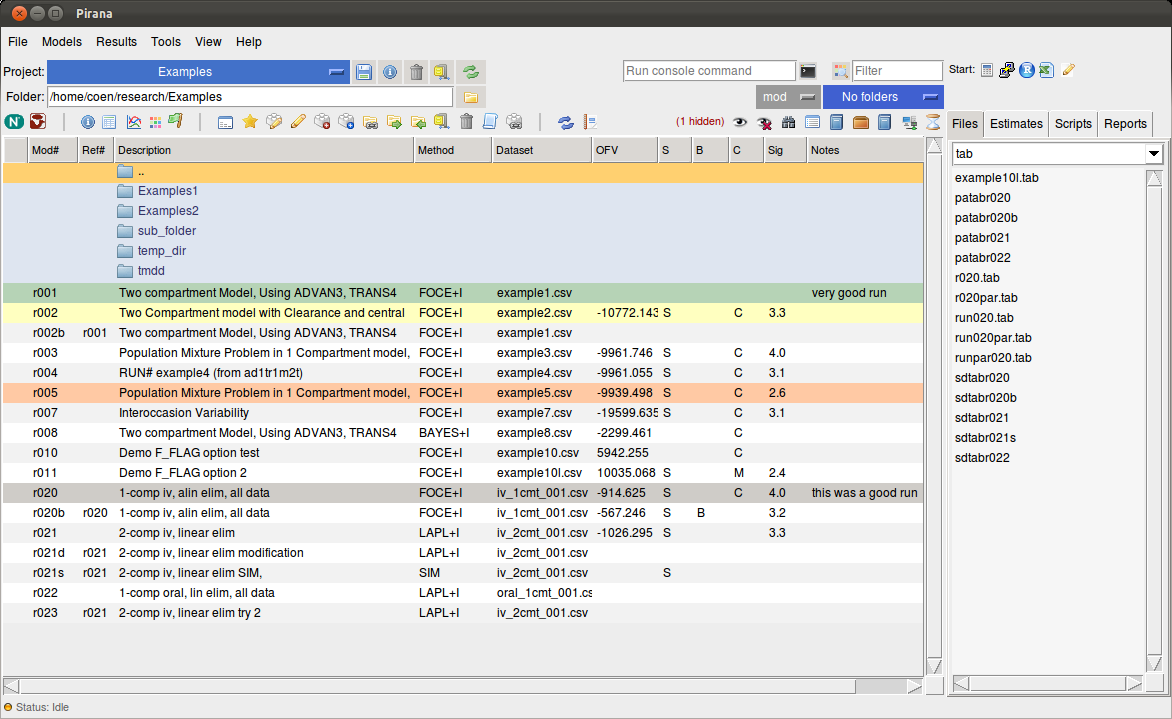
\includegraphics[scale=0.25]{images/pirana_main_screen.png}
    \caption{Pirana main screen (on Linux)}
\end{figure}

\subsection{Model management} The main model overview is
where all models and subdirectories in the current working directory
are displayed. Only models are displayed that have a file-extension
corresponding to the file extension specified in the
\textit{preferences}. If multiple file extensions were specified, choose the
one you want to use in the current folder by selecting it from the listbox
(the one next to the folder selector, on the right above the main models list).
When models are double-clicked, the control stream is opened in the
code-editor (if specified), or else in Pirana's built-in NM-TRAN
editor.

\subsubsection*{Model views}
By default, the model overview is shown as a list, listing all models
ordered by run number. It is assumed models are named as a number
(e.g. '001.mod'), or prepended with 'run' (e.g. `run1.mod', or 'run001.mod'), see
`Conventions and Methods' for more information. By default, the list is shown in \textit{condensed mode},
meaning that for every model, a single row is used in the table. The
list can however also be shown in \textit{expanded mode}, which allows
for longer model descriptions and notes in the overview. Additionally,
in this mode all estimation methods are shown, while in condensed mode
only the last estimation method and associated OFV is shown.

An alternate view mode is \textit{tree view}, in which model development is
shown as a hierarchical tree. The tree is built using parent/reference
information included in the model files (see `run record' explanation in this manual). When creating models in Pirana, this information is added automatically, and adheres to PsN's run record syntax.

The columns that are shown in the main overview can be activated or de-activated from the \textit{View} $\rightarrow$
\textit{Show columns} menu. Models can be filtered using the `Filter' above the
main overview table, or by colors or flags.

\subsubsection*{Model actions}
\noindent New models can be created from scratch, from a template, by
using the Wizards, or by duplicating an existing model:

\begin{description}
\item[Wizards]\ Models can be created by using the PK model
wizard. Choose the desired model type and estimation method, and a
basic NONMEM model file will be created.

\item[Templates] Many basic template models are included. It is
possible to build your own library with base models that you often
use. Templates can be added by copying a model file to
\ttfamily{/templates }\normalfont in the Pirana directory. The
template models should have the same file extension as your model
files to be recognized as a template.

\item[Duplication] Duplication of models can be performed by
selecting the parent model and clicking `duplicate' from the
context-menu (right click on the model). Optionally, final parameter estimates
from the reference model can be updated in the new model, and also
model-file numbers in \$TABLE and \$EST records. Some basic syntax
rules should be adhered to ensure correct interpretation of final
estimates, see Conventions and Methods at the end of this chapter. A
model can also be \textit{Duplicated for MSF restart}. This means that the
model file is duplicated, but an \$MSFI record is added, parameter
estimate blocks are commented out, and the \$MSFO record is updated.

\begin{figure}[H] \centering
    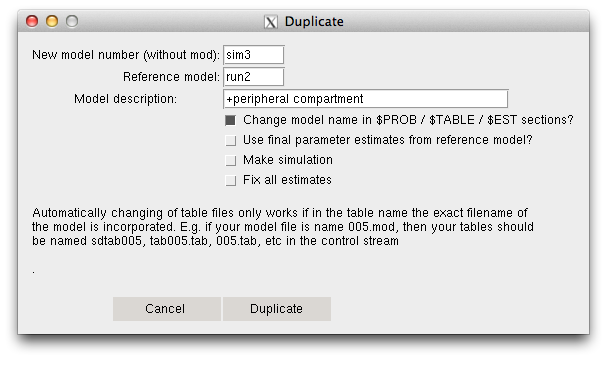
\includegraphics[scale=0.4]{images/duplicate.png}
    \caption{Duplicate model}
\end{figure}

\end{description}

\subsubsection*{Notes, flags and colors}
To each model / run in Pirana, notes can be added. Also, flags and
colors can be added, indicating \textit{key runs}, \textit{good runs},
or \textit{bad runs}. Of course the meaning of the flags and
color-coding is all up to the user. The notes and color info are
stored in a database file (\textit{pirana.dir}), which is created
automatically in each folder that holds models. To add notes to a
model, select the model, right click and select \textit{Model}
$\rightarrow$ \textit{Notes and info}, or using the \textit{Ctrl-I} shortcut. Models and results can be given a color by selecting the model, right-clicking, and selecting the desired color/flag from the \textit{Colors \& flags} submenu. Tip: Pirana supports filtering of models/runs by color.

\vspace{8pt}
\noindent
\scriptsize{
\textcolor{Blue}{Note:} \textcolor{Grey}{In each active folder that
    is visited with Pirana, a small SQLite database is created
    (`pirana.dir') which is able to store information about models. So
    if you archive your projects manually, make sure to include these files as
    well.  }
}
\normalsize

\subsection{Projects} Pirana allows you to save a link to a folder as
a project, which will then be shown in the blue bar (above the active folder
entry). This allows you to quickly switch to the directory that is
linked to that project. To add a project to the list, browse to a
folder by clicking on the folder-icon next to the location bar, or by
clicking through the directory-listing in the model overview. Next,
click on the \textit{disk}-icon next to the project name, give your
project a unique name and press `Save'. Your project is now available
from the listbox. To delete a project from the list, click the trash
icon next to the project list. The green refresh-icon refreshes the
view of the current directory, and should be applied when you make
changes to models or add files outside of Pirana. Also when a run is
finished, you should refresh to gather the results into Pirana.


\subsection{Data files} The list on the right of the screen shows
files in the current folder, if `Files' is selected as the active tab. Pirana can show tab-files, csv-files, R scripts, Xpose files, and other files, which can be selected from the list above. It is also possible to specify your own
filter. Right-clicking on a selected file shows a menu with possible
actions on the file.

\vspace{8pt}
\noindent\scriptsize{\textcolor{Blue}{Note:} \textcolor{Grey}{When the
    Xpose option is chosen, only unique run numbers are shown, instead
    of all tabualar data files. After selecting an Xpose dataset,
    click the `Open in R' the right-click-menu, and R read in the
    datasets and create the Xpose object.  } \normalsize

\section{Working with NONMEM}

There are several ways in which NONMEM can be used from Pirana. The
first one is to use the nmfe-script supplied with NONMEM. For this,
you have to instruct Pirana where NONMEM is installed. The other
(recommended) way to run NONMEM, is to use PsN. When you run NONMEM
through PsN, you don't have to tell Pirana where NONMEM is located,
since this is already specified in the \textit{psn.conf} file of PsN.

\subsection{Managing NONMEM installations} Existing NONMEM
installations can be added to Pirana via the Settings menu, under the
NONMEM tab. Here, both local (upper) and cluster (lower) installations
can be added for use in Pirana. A \textit{smart search} tool is implemented
for local NONMEM installations, which searches for NONMEM
installations in the most common locations on your local drives. If
you have installed NONMEM in a non-common location, or want to use
NONMEM on a remote cluster, add the paths to NONMEM manually.

\begin{figure}[H] \centering
    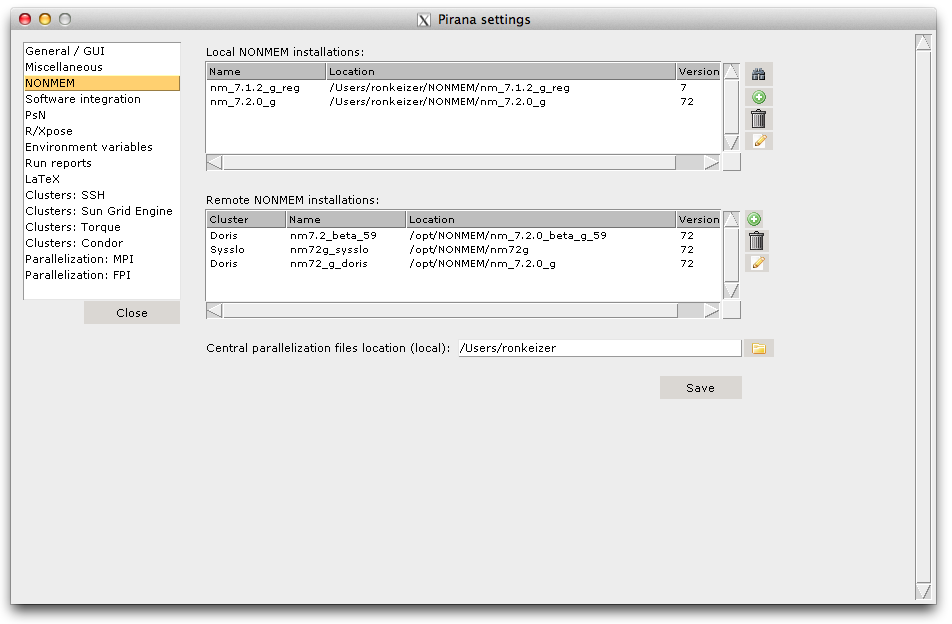
\includegraphics[scale=0.31]{images/nonmem_settings.png}
    \caption{NONMEM settings window}
\end{figure}

\subsection{Setting environment variables}
NONMEM requires a Fortran compiler installed. For
this compiler to function properly, it is important to set the
environment variables correctly. Especially for Intel compilers, this
can be trooublesome, as different environmental variables need to be
defined. For GNU compilers, setting the PATH environment variable is
usually sufficient. There are several ways you have control over the
environment variables when using Pirana:

\begin{enumerate}
\item In the settings menu, under \textit{Environmental variables},
  the PATH variable used within the Pirana environment can be defined,
  or additional folders can be added to the existing PATH. Also,
  additional environmental variables can be defined here.

\item Alerntatively, in the same settings screen for each nmfe-run
  that is started, you can specify a command that will be executed
  before starting nmfe-type runs, which can be e.g.

\begin{lstlisting}
  PATH=%PATH%;C:\gfortran\bin
\end{lstlisting}

\item At startup, Pirana will check for the existence of 2 files in
  the Pirana base folder: \textit{set\_env.txt} and
  \textit{add\_env.txt}. These files can be used to either set, or add
  to the system variables, respectively. The files may look e.g. like
  this:

\begin{lstlisting}
PATH=C:\nmvi\run;C:\MinGW\bin
VARX=C:\bladibla;etc
\end{lstlisting}
\end{enumerate}

\clearpage
\subsection{Running models}
As mentioned before, a model can be run using \textit{nmfe} directly, \textit{PsN} or
\textit{WFN} (Windows only). This can be done by selecting a model from the list, and
right-clicking to show the context-menu.  From here, you can either
select NONMEM-nmfe, or the PsN or WFN options. The commands are also
available from the toolbar. WFN is disabled by default.

\subsubsection*{Using nmfe}
Execute a model using `Run (nmfe)', or press Control-R. This will open up a
dialog showing two additional options
for running the model, e.g. which NONMEM installation to use, and if
models should be executed in separate folders or on a cluster system.

\begin{figure}[h] \centering
    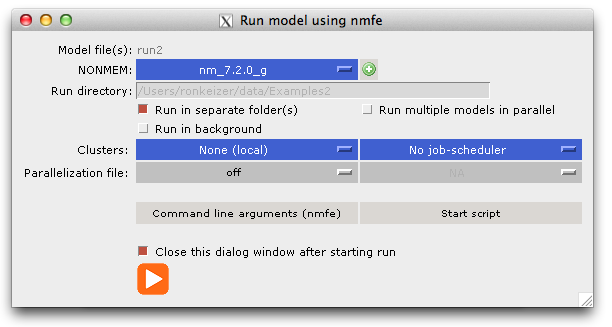
\includegraphics[scale=0.5]{images/nmfe_run.png}
    \caption{nmfe run window}
\end{figure}

\noindent Pirana supports the use of the parallelization functionality available
in NONMEM 7.2. When you select a NONMEM 7.2 installation in the nmfe
run window, the available parallization files (\textit{parafiles}) are displayed under the parallelization tab. \textit{Parafiles} can be generated using the Wizard in Pirana. You can also have Pirana generate the \textit{parafile} on-the-fly (select \textit{auto-MPI} or \textit{auto-FPI}). Under Settings $\rightarrow$ Parallelization, the FPI and MPI files that Pirana generates can be specified.

\vspace{5pt}

\noindent Parallization files can be imported from local or remote locations. Local import can be performed through Settings $\rightarrow$ NONMEM. Remote parallelization files can be imported from a cluster location defined under Settings $\rightarrow$ SSH.

\begin{figure}[H] \centering
    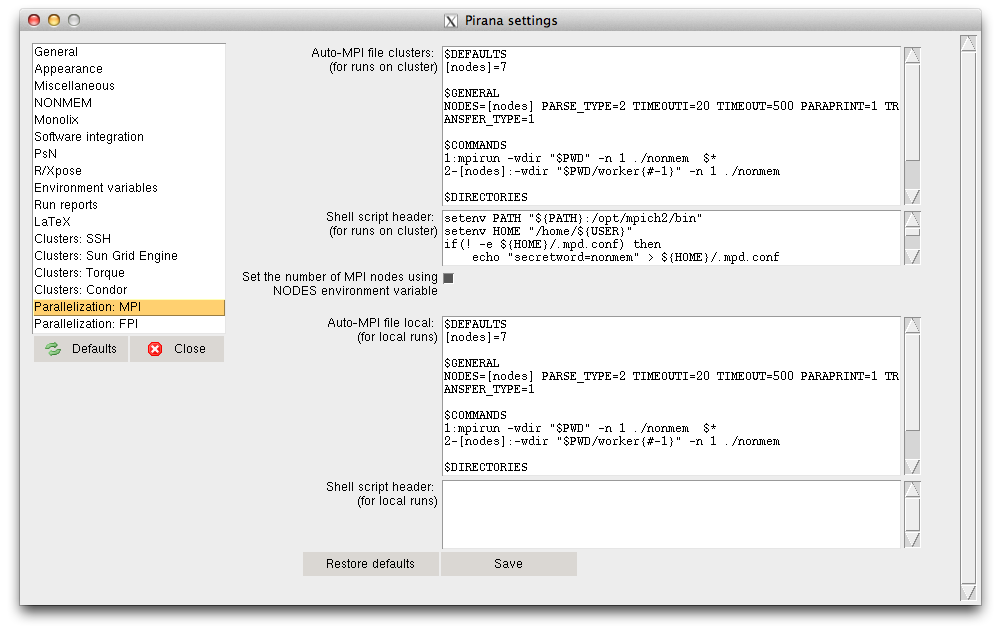
\includegraphics[scale=0.27]{images/settingsparallization.png}
    \caption{Automatic parallelization file}
\end{figure}

\clearpage

\subsubsection{Using PsN}
PsN is an extensive toolkit for advanced modeling \& simulation, and
contains essential tools such as bootstrapping, visual predictive
checks (vpc), stepwise covariate modeling (scm), simulation and
re-estimation (sse), and many more. All PsN-toolkit functions can be
accessed from Pirana using the right-click menu or the toolbar. \textit{Execute} is
also conveniently available using the Ctrl-e keyboard shortcut. The
dialog window is then opened (shown below), which can also shows the
PsN-help info for the selected command. The command line editor can be
used to specify additional parameters to the PsN funtion. Pirana
stores each executed PsN command, which are available from the
'History' button.

\begin{figure}[H] \centering
    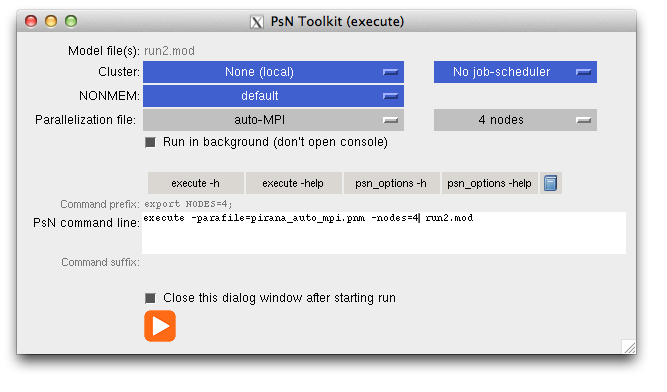
\includegraphics[scale=0.42]{images/Figure2_4_PsNdialog2.png}
    \caption{PsN dialog window}
\end{figure}

\noindent From the PsN tab in the Settings window you can define the default
command line parameters for most PsN functions. Some of PsN's functions are not related to models, but to datasets, such as data\_stats, \textit{create\_subsets} etc. These functions can be invoked from the file list on the right by selecting a file and opening the menu by right-clicking the mouse. A similar interface will be opened
as for PsN's model functions.

Similar to the nmfe dialog window, the PsN dialog also offers the possibility to
easily setup parallel execution. Pirana can be instructed to auto-generate
the MPI/FPI file required for parallel execution. When MPI or FPI, and the number of nodes are selected,
Pirana will automatically add the required PsN arguments ({\tt -parafile} and {\tt -nodes}).

\subsubsection*{Using Wings for NONMEM}
On Windows, Pirana is
capable of invoking the WFN-commands \emph{nmgo} and \emph{nmbs}, for
run execution and bootstrapping respectively. Since
WFN does not support multiple model files to be processed by its
commands, when multiple models are selected, only the first model file
is executed. When the WFN method is selected, two parameter
specification bars will become visible. In the upper entry, run
parameters can be specified, e.g. for the bootstrap: `1 100' to
specify a bootstrap with 100 replicates. The lower parameter bar
specifies command-line parameters used when starting WFN.bat,
e.g. `g77 std' for specifying the compiler and the NONMEM version to
be used.

\vspace{10pt}
\noindent\scriptsize{\textcolor{Blue}{Note:} \textcolor{Grey} {What Pirana actually does when executing runs through WFN, is create a temporary batch-file in the current directory that starts \emph{WFN.bat} to load the necessary environment variables, after which \emph{nmgo} is started with the model-file and parameters specified.}
  \normalsize

\clearpage
\section{Analyzing results \& output}

\subsection{Main overview}
After a model has been run/executed, and the folder is refreshed, Pirana will show the main results of the run in the main overview. It will show the OFV, the difference in OFV with the reference model (if specified), the number of significant digits, and some information about the estimation, i.e.:
\begin{description}
\item [S] means a succesful minimization (as reported by NONMEM)
\item [R] means estimation ended with rounding errors
\item [C] means a succesful covariance step
\item [M] means an unsuccesful covariance step due to matrix singularity
\item [B] means a boundary problem was reported by NONMEM
\end{description}
Pirana can also show the AIC and BIC values for the model, although these have to calculated first. See `Miscellaneous functionality' in this manual for more information.

\subsection{Parameter estimates}
A list of parameter estimates is shown in the right section of the Pirana window,
if `Estimates' is selected as the active tab. It also shows the RSE for parameters (between round brackets),
and shrinkage for the random effects (between square brackets). In this overview it is also highlighted if
final gradients for a parameter were zero (red foreground), mean of eta-distribution was significantly different from zero (etabar, red background), boundaries were encountered (blue background), or parameters were fixed (grey background).
A more detailed list is available by selecting \textit{Models $\rightarrow$ Parameter estimates} from the right-click menu, or from the toolbar. If just
one model is selected, Pirana will show all parameter estimates and
associated RSE values, if available. If multiple models/runs are
selected, Pirana will show the parameter estimates of these runs side
by side, facilitating comparison. These results can be easily
converted into CSV, LaTeX or HTML for e.g. reports or further
analysis. The estimates can be exported by R as well, by clicking the
R-icon in the parameter estimates area.

\begin{figure}[H] \centering
    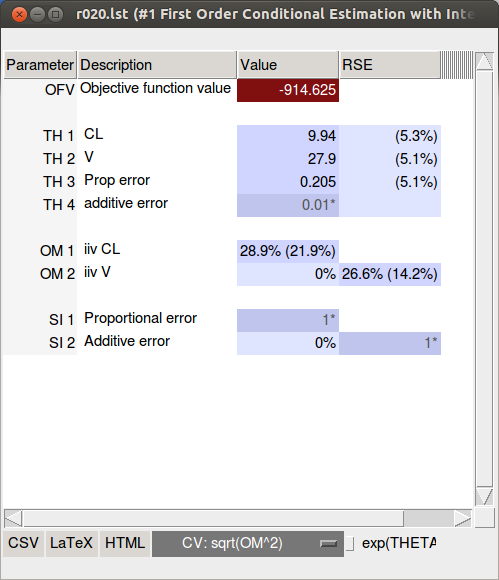
\includegraphics[scale=0.3]{images/estimates_window.png}
    \caption{Parameter estimates window: Single run}
\end{figure}

\begin{figure}[H] \centering
    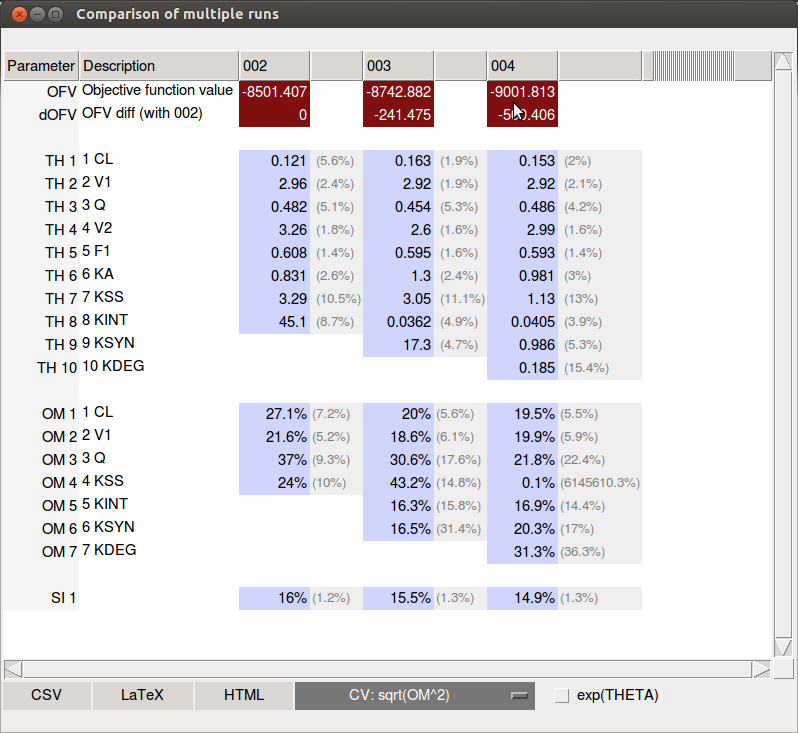
\includegraphics[scale=0.3]{images/compare_estimates.png}
    \caption{Parameter estimates window: Comparing multiple runs}
\end{figure}


\subsection{Run Reports} Run reports with model and run info, and parameter estimates can automatically be generated, and outputted as HTML, \LaTeX \hspace{2pt},
Word, or plain text format. The reports optionally displays basic run
information, run statistics, description and notes, and parameter
estimations, split by implemented estimation methods. The information to
be included in the report can be specified in the menu under `Settings
$\rightarrow$ Run reports'. \LaTeX \hspace{2pt} output is opened in
the specified code editor, but also can be converted automatically to
PDF using pdflatex (if installed).\\

\noindent After a run report is generated it will show up in the list
on the right, under the tab \textit{Reports}. In this tab, also
goodness of fit plots are shown, generated either using the Xpose GUI
in Pirana, or the R scripts library. Double-clicking on any of the
plots or reports will re-open them.\\

\vspace{10pt}
\noindent\scriptsize{\textcolor{Blue}{Note:} \textcolor{Grey} {In the
    run reports, Pirana calculates the RSE for population parameters
    as $RSE_{\theta_i} = \frac{SD_{cov,\theta}}{\theta_{i}}$, but doesn't take into account
    log-transformation of parameters (e.g. when MU-modeling). For
    inter-individual and residual variance ($\Omega$ and $\Sigma$),
    RSE's are calculated as e.g. $RSE_{\omega_{i,i}^2} =
    \frac{SD_{cov,\omega_{i,i}^2}}{\omega_{i,i}^2}$. RSE's given for
    $\omega_{i,i}$ and $\sigma_{i,i}$ are calculated as e.g. $RSE_{\omega_{i,i}} =
    \frac{SD_{cov,\omega_{i,i}^2}}{2 \cdot \omega_{i,i}^2}$ } \normalsize
\vspace{10pt}

\subsection{Intermediate results} When running models through any of
the available methods (nmfe / PsN / WFN), the intermediate results
(parameter estimates, objective function value, gradients) can be
viewed by clicking on the \textit{hourglass}-icon or from
\textit{Tools $\rightarrow$ Intermediate results}. This will open a
window which shows the models that are currently running. By clicking
on a run in the list, Pirana will parse the intermediate files and show the intermediate parameter estimates in the table and the plot. In the plot, you
can choose to show either the gradients (if a gradient method is
used), the intermediate estimates, or the objective function value
(OFV). Make sure that you specify PRINT=1 and MSFO=xxxxx in the
\$ESTIMATION record, to be able to obtain regularly updated
intermediate estimates. From the right-click menu, signals can be
sent to currently running NONMEM processes, such as \textit{stop} and
\textit{next iteration}.

\begin{figure}[H] \centering
    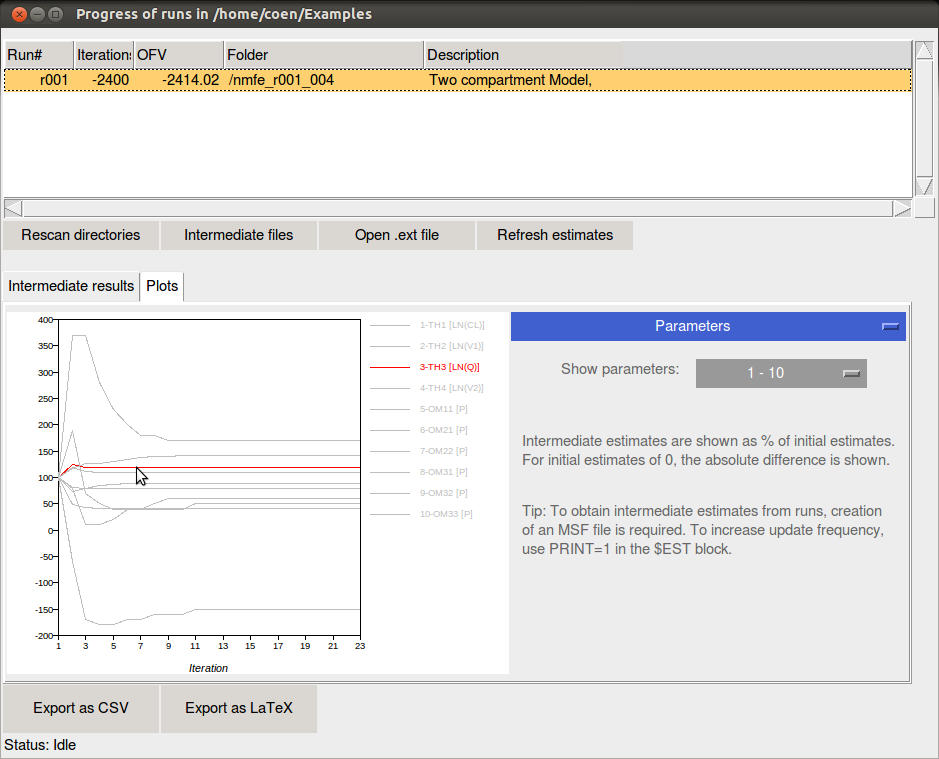
\includegraphics[scale=0.3]{images/intermed.png}
    \caption{Intermediate results}
\end{figure}

\subsection{Run Records}
For all models in the current folder, or a selection thereof, a CSV
run record can be compiled by Pirana that includes all
model and run characteristics, such as model description, estimation
method, objective function value, termination result, etc. An abridged
version of the run record can also be created as a plain text or Word
document.

\subsubsection*{Visual Run Record}
Pharmacometric model development most often progresses in a
hierarchical fashion, using the likelihood ratio test to assess
significance of improved fit between nested models. An appropriate
visualization of the model hierarchy will help the modeler gain better
understanding of key stages in model building, and willl aid in
communicating the model development history to others. Such a
visualization can be generated by Pirana, an example of which is shown below.

\begin{figure}[H] \centering
    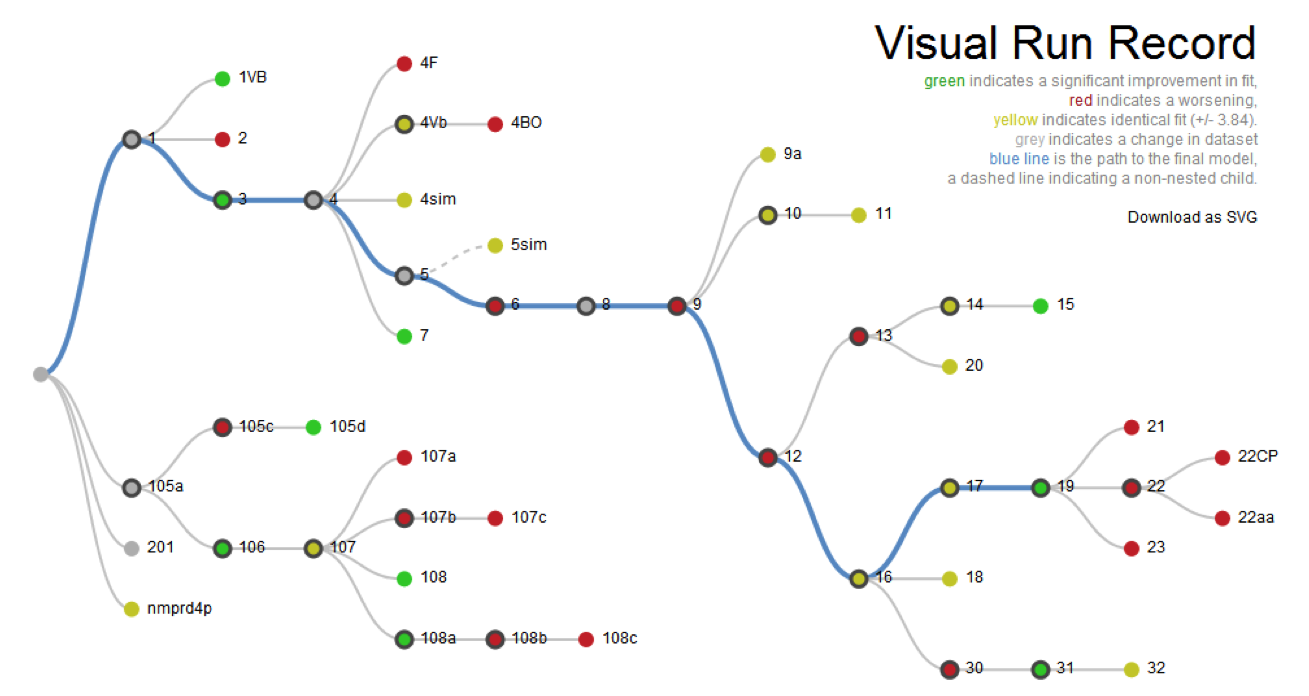
\includegraphics[scale=0.47]{images/vrr.png}
    \caption{Visual Run Record}
\end{figure}

\noindent To create the VRR, Pirana produces Javascript code compatible with the Data-Driven
Documents Javascript library (d3.js). The visualization can be
generated as an SVG image in any modern internet browser. Several
options are implemented that allow customization of the visualization,
and both dynamic and static images can be created. In a VRR, the
hierarchy of models is immediately visible, and using the dynamic
collapsable dendrograms, non-relevant model threads can be hidden from
the visualization. The VRR also shows additional model information
when hovered over the nodes. Colors aid in visualizing the improvement
/ worsening of model fit (green / red), and whether the model has
children or not. In each branch, the nodes are ordered by OFV. When a
final model is specified, the modeling path can be made visible as a
blue line, thereby easily identifying the key runs. The visualization
can be implemented as a horizontal or radial tree, the latter of which
can be used when the model tree is very large.

\subsection{Data Inspector} Pirana is able to construct scatter plots
using the built-in \textit{DataInspector}, e.g. for quickly inspecting
goodness-of-fit, covariate relationships, distribution of etas,
performing data checkout etc. The DataInspector shows all the columns
present in the dataset, which can be mapped to the X- or Y-axis
(shown in figure 3.2). DataInspector can either be invoked by
selecting a model (main overview), or a data file (from the list on
the right). If a model is selected and DataInspector is started,
Pirana will gather the dataset specified in \$INPUT and the table
files created in \$TABLE. It will then ask the user which of these
files to open in DataInspector. If only one file is found, it will
open that one automatically.

\begin{figure}[H] \centering
    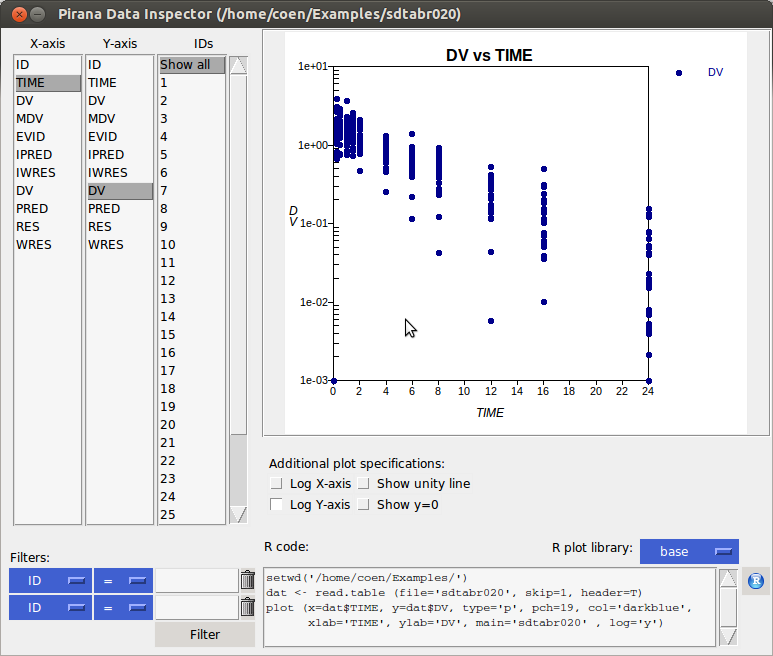
\includegraphics[scale=0.35]{images/plot.png}
    \caption{Pirana DataInspector}
\end{figure}


  \subsection{Visual run records}
The model building process from initial to final model can be visualized using the visual run record.
This can be done via Results  $\rightarrow$ Run records $\rightarrow$ Visual run record.
Here a final model can be selected, and the visual run record will be graphically depicted.

  Pirana can parse NONMEM-generated tables, and CSV-files. Multiple Y values
  can be plotted by holding the Control- or shift-key and selecting
  multiple (up to three) data columns. Inside the plot, regions of
  interest may be selected, which are then zoomed. Double-clicking
  inside the plot region changes back to the previous view. Plots can
  be filtered, which can be useful, e.g. to show only data for one
  patient, or groups of patients or covariates.

  In the text-box below the plot, code is generated that recreates
  the same graph in R, either in \textit{base}, \textit{lattice}, or
  \textit{ggplot2}. This code can be used as a starting
  point for the generation of plots for manuscripts or
  reports. Clicking the `R'-button will invoke the R-GUI or code
  editor.

\subsection{R scripting for creating graphs and file processing}
Pirana includes functionality to run custom R-scripts on output from
models-executions such as NONMEM tables. Scripts can be written by the
user, but a considerable collection of scripts is also bundled with
Pirana, which can serve as starting point for your own
implementations. Scripts are located in three locations, one for
group-wide scripts (in the scripts-folder in the location where Pirana
is installed), one for user-scripts (`home/user/.pirana/scripts'
on Linux, `C:$\backslash$Documents and
Settings$\backslash$user$\backslash$Application
data$\backslash$.pirana$\backslash$Scripts' on Windows), and one for project-specific scripts, stored in the subfolder pirana\_scripts in the current folder. The folder
structure underlying the scripts folders is reconstructed within the
scripts menu, and scripts can be edited either by editing them from
outside Pirana, or by choosing them from the `Edit' menu option.

Scripts can be started by selecting a model, and selecting the desired
script from the scripts menu located in tight tab panel. Pirana invokes R and runs the script in the
directory `pirana\_temp' underlying the active folder.  However,
before execution, Pirana replaces \textit{\#PIRANA\_IN} with an R
list-object which specifies model and results information, e.g. as:

\begin{lstlisting}
models <- list (
   "003" = list (
     "modelfile"       = "003.mod",
     "description"     = "PK model digoxin",
     "reference_model" = "002",
     "data_file"       = "nm_pk_001.csv",
     "output_file"     = "003.lst",
     "tables"          = c("003.TAB", "sdtab003")
   )
 )
\end{lstlisting}

\vspace{15pt} \noindent To automatically load PDFs or images that are created by
R after execution of the script, you should include e.g. the following line in
the script:

\begin{lstlisting}
#PIRANA model_output.pdf
\end{lstlisting}

\noindent where model\_output.pdf is the file that you want Pirana
to load. This may either be a PDF, or a common image format such as
PNG, JPG, or GIF. Please have a look at the scripts included with
Pirana for examples this
functionality.

\vspace{10pt}
\noindent\scriptsize \textcolor{Blue}{Note:} \textcolor{Grey} {
By default, R scripts started from Pirana will run in the same \textit{thread} as the main Pirana program. However,
for scripts that require long processing time this can be problematic, since Pirana cannot be used during
the execution of the script. If the following code is added somewhere in the R script, the script
will be run in a separate console instead and not block Pirana itself:}

\begin{lstlisting}
#PIRANA_NEW_CONSOLE
\end{lstlisting}

\normalsize

\subsubsection*{Interactive scripts}
From Pirana 2.6.0 onwards, Pirana has the ability to create
\textit{interactive scripts}, meaning that upon execution of an
R-script, the user will be presented with an
interface that shows plotting and input options. The plotting options can be
specified in the R-script like e.g.:

\begin{lstlisting}
### <arguments>
###       <title label="Plot title">DV vs PRED</title>
###       <x_var label="X-variable">DV</x_var>
###       <xlab label="x-axis label">Dependent variable</xlab>
###       <y_var label="y-variable">PRED</y_var>
###       <ylab label="y-axis label">Pred. concentration</ylab>
###       <subset label="Subset string"></subset>
###       <split_id label="by ID" type="bool">FALSE</split_id>
### </arguments>
\end{lstlisting}

\vspace{4pt}

\noindent This will result in the following interface:

\begin{figure}[H] \centering
    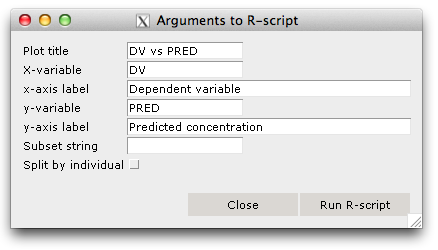
\includegraphics[scale=0.5]{images/interactive_scripts.png}
    \caption{Interactive scripts}
\end{figure}

\noindent In the R-script, the specified options are then available
as the list \textit{arg}, e.g using:

\begin{lstlisting}
ggplot (data=tab, aes (x=get(arg$x_var),
                       y=get(arg$y_var))) + geom_point()
\end{lstlisting}

\subsection{Xpose support}
After selecting a model, Xpose can be invoked from the scripts menu either by
selecting the integrated Xpose GUI or the calling the (external) Xpose R-menu.
The integrated Xpose GUI allows for execution of Xpose commands. The user can also add
optional arguments to Xpose commands.  Plots can be saved as PDF or
PNG files, or Sweave/knitr code can be generated.

\begin{figure}[H] \centering
    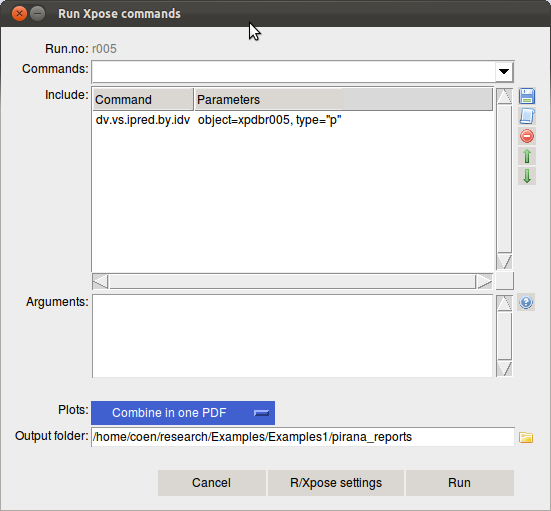
\includegraphics[scale=0.5]{images/xposewindow.png}
    \caption{Xpose window}
\end{figure}

\noindent Besides the commands available in the list, you can also input your
own commands or statements to the list. Lists can be saved for easy
access later on. The general plotting arguments for PDF and PNG
(e.g. {\ttfamily width=10, height=8} can be set in the settings menu
under \textit{R/Xpose})

\subsection{Wizards}
As mentioned earlier, Pirana comes with several wizards, such as a
wizard to create a NONMEM model file, PsN-scm configuration files, and
parallelization files. You can alter these Wizards to your liking, as they are
implemented from wizard-specification files located in
\textit{/wizards} in the Pirana installation folder. Of course, it
is possible to create your own Wizards as well. Just create a
\textit{.pwiz} file in the wizards-folder and follow the instructions
in the template that is provided there. Wizards that are included with
the current version of Pirana are described below:

\subsubsection*{PK model}
This wizard allows stepwise construction of a range of PK models in
NONMEM. It includes all ADVANs in NONMEM, all estimation methods, and
the most commonly used residual error models. Of course, keep in mind
that you have to change the initial estimates and the \$DATA and
\$INPUT records to suit your PK problem.

\subsubsection*{NM parallelization file}
NONMEM 7.2 and higher allow parallization of single runs, which
requires a so-called `parafile', a configuration file for the
parallelization. These files can be created using this wizard.

\subsubsection*{SCM configuration file (PsN)}
The scm command in PsN requires a configuration file. With this wizard
you can create such a file, which includes the most commonly used
options. Please note that more features are available in the scm tool
than are offered as option in the Wizard, so it is advised to acquaint
yourself with the full scm documentation.

\subsubsection*{Dataset template}
This wizard can be used to create an R script that, in turn, generates
a NONMEM simulation data file with specified number of individuals,
doses, observations, dosing times, and covariates. This can be useful
e.g. for quickly setting up simulations in NONMEM.

%%%%
\section{Model translation}
Pirana can translate NM-TRAN models written in any ADVAN routine to
ordinary differential equations (ODEs). The model can be exported to
ADVAN6 (NM-TRAN), to R (using the deSolve library), Berkeley Madonna,
MATLAB and PopED. Also several translators are included that
translate specific parts of NONMEM code to alternate NONMEM code.

\subsubsection*{Translation to other tools}
For R, a multidose simulation is automatically implemented, for the
other converters only single dose simulation is implemented. Pirana
currently does not read in the dataset to extract dosing information.

Pirana extracts the parameter estimates for the structural model
($\theta$), and also the between subject variability matrix
($\Omega$). The latter is however done only when simulating in R or Berkeley Madonna (not available for Matlab at current).
No residual error model is currently implemented in any of the translators, but this can easily be added by the user.

Porting the model structure to PopED allows evaluation of optimal
study designs (OD). Pirana creates the necessary files for PopED execution, however
the user still needs to provider the details of the design and other optimization settings.

\subsubsection*{MU-model conversion}
Pirana can convert standard NONMEM models to MU-model coding. At
current, Pirana can only convert models written using normal- or
log-normal $\eta$s, e.g.

\begin{lstlisting}
CL = THETA(1) * EXP(ETA(1))
\end{lstlisting}

will be converted into:

\begin{lstlisting}
MU_1 = LOG(THETA(1))  ; ** MU-referenced by Pirana
CL = EXP(MU_1+ETA(1))
; Original equation: CL = THETA(1) * EXP(ETA(1))
\end{lstlisting}

\subsubsection*{Difference equations}
For some models written in ODEs, writing some parts of the model in
difference equations can considerably reduce computational burden, while
maintaining parameter precision.\footnote{Petersson KJ et al. J
  Pharmacokinet Pharmacodyn. 2010 Oct;37(5):493-506.} Pirana can help
in setting this up: it will transport all code written in \$DES other
than the $\frac{dA}{dt}$ system to \$PK, and adds some required
code (using \textit{MTIME}).

\section{Batch operations}

Pirana offers functionality to perform batch operations on a set of
models, such as search and replace functions.

\begin{description}
	\item{\textcolor{Grey}{Search and replace in models}} Replaces
          a given search text with another string or block of text in
          the selected models.
	\item{\textcolor{Grey}{Replace block}} This function enables
          you to replace a whole block of code in selected model
          files, e.g. the \$DATA block if you want all model files to
          use a different data file, or the \$THETA block if you want
          to use other initial estimates.
	\item{\textcolor{Grey}{Add code to models}} With this
          function, lines of code can be added to the beginning or the
          end of selected models.
	\item{\textcolor{Grey}{Add code to blocks}} With this
          function, lines of code can be added to a specific block in
          the selected models.
	\item{\textcolor{Grey}{Batch duplicate}} Creates multiple
          duplicates of one model file, with (optionally) updated
          run/table numbers and final parameter estimates.
	\item{\textcolor{Grey}{Random simulation seeds}} In all
          selected models, the \$SIMULATION block will be updated with
          new seeds.
\end{description}

\section{Miscellaneous  functionality}

\subsubsection*{NONMEM help files}
Modeling with NONMEM, and construction of NM-TRAN syntax can be
troublesome at times, and therefore it is convenient to have NONMEM's
help files at your fingertips. Pirana provides a user interface to
these help files, allowing you to filter on keyword. Before help file
interface can be used, the NONMEM help files need to be imported as
the files are not supplied with Pirana. For this, go to `Tools'
$\rightarrow$ `NONMEM' $\rightarrow$ `Import / update NONMEM help
files' to perform this. You can import the information from a local
NONMEM installation or from an installation located on a cluster (over
SSH). After succesful import, the NONMEM help interface is availabe
from the `Help' menu.

\subsubsection*{Code differences between models}
Pirana provides a tool to show code differences, similar to the
\textit{diff} functionality on Unix systems. If one model is selected
and the diff tool is activated (Right-click menu $\rightarrow$
`Model' $\rightarrow$ `Code difference between models'), Pirana will
show the difference between that model and the reference mode (if
specified). If two models are selected, Pirana will show the code
differences between these two models.

\begin{figure}[H] \centering
    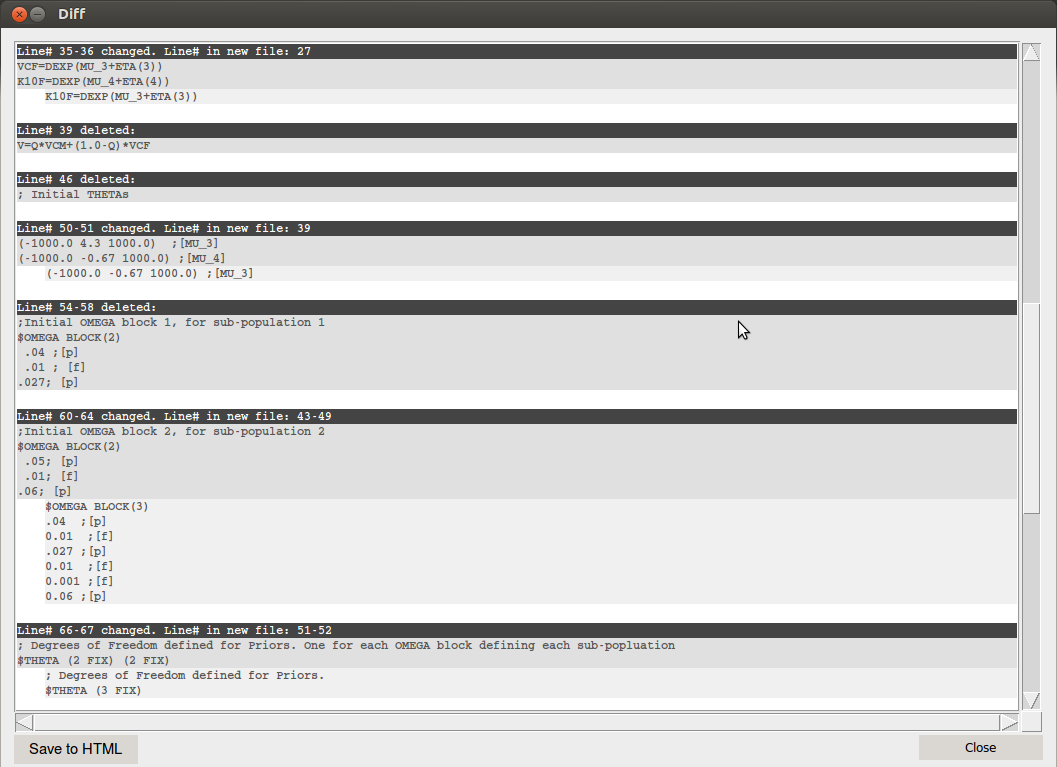
\includegraphics[scale=0.28]{images/diff.png}
    \caption{Code difference between models}
\end{figure}

\subsubsection*{Model Archive: Automatic backup of models and results}
When editing and running models, Pirana can automatically backup all
versions of controlstreams and result files. When this feature is
activated (in the settings menu), intermediate versions of models and
results are saved in a separate folder, every time a model is changed,
or when a new results files is found. The archive can be accessed via
the \textit{Tools} menu, under the option \textit{Model
  Archive}. Details of the run and (if applicable) parameter estimates
can be reviewed. Also, different versions of models can be compared
and restored. The internal Pirana database files (\textit{pirana.dir})
are also backup up, if it has been more than a week since the previous
backup.

\begin{figure}[H] \centering
    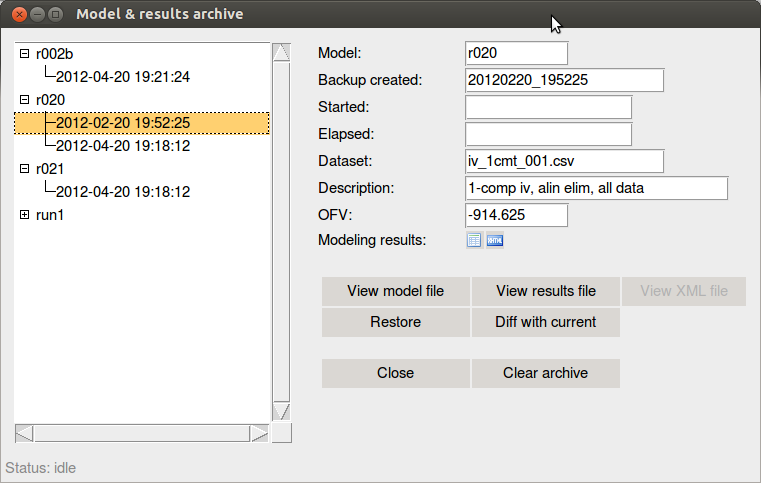
\includegraphics[scale=0.35]{images/modelbackup.png}
    \caption{Model backup / archiving window}
\end{figure}

\subsubsection*{Matrices}
Pirana can automatically extract the covariance, correlation and
inverse covariance matrices from a NONMEM 7+ run (cor/cov/coi files),
and show them in a spreadsheet-like window. These can then also be
automatically exported to an R object, for instance for simulation
purposes.

\begin{figure}[H] \centering
    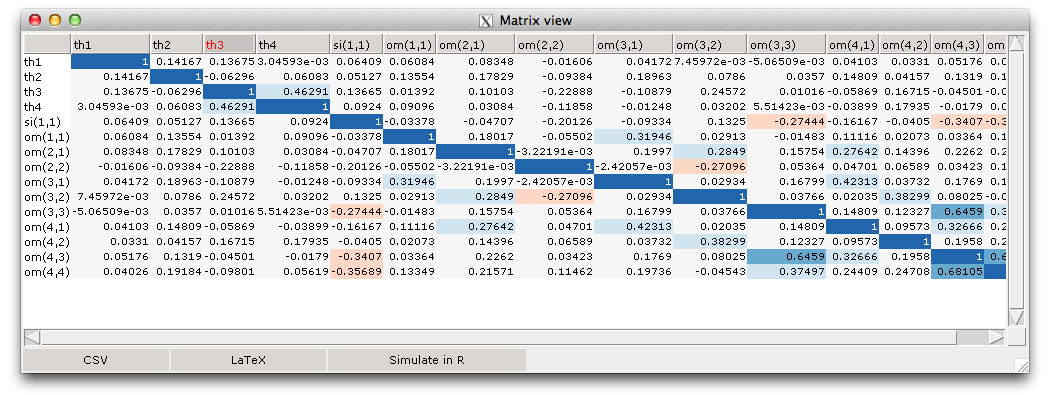
\includegraphics[scale=0.28]{images/cor.png}
    \caption{Correlation matrix}
\end{figure}

\subsubsection*{Miscellaneous tools}

\begin {description}
  \item{\textcolor{Grey}{Correlation calculator}} This opens the
built-in `Correlation Calculator', which can be used to re-calculate a
covariance to a correlation on the SD-scale. The formula for
correlation that is used is:

\vspace{10pt}
$ \rho_{i,j} = \frac{{\omega_{i,j}}^2 }{\omega_{i,i} \cdot \omega_{j,j} }
$
\vspace{10pt}

with $\rho$ specifying the correlation between two elements (i,j) in a
matrix, and $\omega$ specifying elements of $\Omega$ or $\Sigma$.

  \item{\textcolor{Grey}{Checkout dataset}} This will create (and open)
an HTML-file which displays a selected dataset using separate colors for
different event-types. This will thus show the dataset in a slightly more
convenient format for manual inspection than in a spreadsheet. The
function needs at least the ID, TIME and EVID columns in the dataset to work properly.

  \item{\textcolor{Grey}{Calculation of AIC/BIC}} Pirana can calculate
    the Akaike Information Criterion and the Bayesian Information
    Criterion. These criterions are defined as follows:

\begin{equation}
AIC = 2 \cdot k - 2 \cdot ln(L)
\end{equation}

\begin{equation}
BIC = -2 \cdot ln(L) + k \cdot ln(n)
\end{equation}

with $k$ the number of parameters in the model, $L$ the maximized
value of the likelihood function, and $n$ the number of observations
in the dataset used in fitting the model. The calculation of these
criterions is however not so straightforward for non-linear mixed-effects
models, and the weights/penalties applied to parts of the equation can
be different in different circumstances. Pirana allows the penalties
to be changed when it calculates the AIC/BIC. From the right-click
menu, select \textit{Model actions} $\rightarrow$ \textit{Calculate
  AIC/BIC}, and a dialog window will open which will present the
options available. Some useful literature is listed below.

\scriptsize
\begin{itemize}
\item Vaida and Blanchard, Conditional Akaike information for
mixed-effects models. Biometrika, 2005. 92(2): p. 351-370.
\item Liang, et al., A note on conditional aic for linear
mixed-effects models. Biometrika, 2008. 95(3): p. 773-778.
\item Hodges and Sargent, Counting degrees of freedom in hierarchical
  and other richly�]parameterised models. Biometrika (2001) 88 (2): 367-379.
\item Donohue et al., Conditional Akaike information under generalized
  linear and proportional hazards mixed models, Biometrika (2011) 98
  (3): 685-700.
\item Delattre et al., BIC selection procedures in mixed effcts
  models \\ http://hal.inria.fr/docs/00/69/64/35/PDF/RR-7948.pdf
\end{itemize}
\normalsize

\item{\textcolor{Grey}{Clean-up folder}} This tool can be used to
  clean-up files that NONMEM generates when running a model (e.g
  INTER, FSTREAM, etc.). So if you run a model in the main model
  folder (which is not considered good modeling practice),
  you can use this tool to clean up after model execution.

\end{description}

\clearpage
\section{Conventions and Methods}
\subsubsection{Model file conventions}

\begin{itemize}
\item Users of PsN and Xpose likely follow the `Uppsala convention' of
  having model files named like \textit{run1.mod}, \textit{run2.mod},
  etc. This is recommended for Pirana users as well, although
  Pirana is flexible in this respect. Note that Pirana removes
  the 'run' from the modelfile name in the model overview.
\item Pirana looks for a description of the model in the first part of
  the model file. It adheres to PsN's run record standards.
  If the PsN run record is not used,
  Pirana searches for the words `\ttfamily{\$PROBLEM}' \normalfont or
  `\ttfamily{Model desc:}' \normalfont to extract the model
  description.
\item If you want to use the hierarchy functionality for models, you
  should specify the reference model in the first few lines of the
  model file. Again, best is to use PsN's run record specification, but
  Pirana is flexible and also compatible with Census, and
  understands the following syntaxes:

\begin{lstlisting}
;; 1. Based on: 001.mod
; Ref. model:001.mod
; Ref:001.mod
; Parent=001.mod
\end{lstlisting}

\item Model parameter descriptions need to be specified
after a semi-colon, e.g.

\begin{lstlisting}
$THETA
(3, 5, 11) ; CL/F
(10, 50, 100) ; V/F
\end{lstlisting}

Note that Pirana reads these decriptions from the model file (and
not from the output file). To be read correctly, covariance block need
to be specified as:

\begin{lstlisting}
$OMEGA BLOCK(2)
0.1 ; IIV CL/F
0.05 ; COV CL~V
0.1 ; IIV V/F
\end{lstlisting}

or as:

\begin{lstlisting}
$OMEGA BLOCK(3)
0.1           ; IIV CL/F
0.05 0.1      ; IIV V/F
0.01 0.05 0.1 ; IIV KA
\end{lstlisting}

\item When models are to be executed in a separate directory, files
  needed for compilation (e.g. additional Fortran routines in .FOR
  files), are copied automatically by Pirana. These files should be
  specified in the \ttfamily{OTHER} \normalfont and \ttfamily{CONTR}
  \normalfont entries on the \ttfamily{\$DATA} \normalfont record. If
  more additional files are needed, you can instruct Pirana to copy
  these by adding this line to your control stream:

\begin{lstlisting}
; INCLUDE=file1_to_be_copied.ext,file2_to_be_copied.ext,etc
\end{lstlisting}

Note that PsN has it's own functionality for doing this.

\end{itemize}

\section{Keyboard shortcuts}
The following keyboard shortcurts are available in Pirana:
\begin{itemize}[noitemsep,topsep=5pt,parsep=1pt,partopsep=0pt]
  \item        Ctrl-R: Run model
  \item        Ctrl-L: Open NM output file (.lst)
  \item        Ctrl-N: New model file
  \item        Ctrl-D: Duplicate model file
  \item        Ctrl-P: Show parameter estimates for run(s)
  \item        Ctrl-T: HTML-file from NM output
  \item        Ctrl-E: Execute model (PsN)
  \item        Ctrl-B: Bootstrap model (PsN)
  \item        Ctrl-V: VPC from folder (PsN)
  \item        Ctrl-U: Update inits (PsN)
  \item        Ctrl-X: Run Xpose commands
  \item        Ctrl-A: Select all models
  \item        Ctrl-+/-: Increase / decrease font size
  \item        Ctrl-, : Open settings window
  \item        F5 : Refresh current folder
\end{itemize}

\clearpage
\section{Command line parameters}

\begin{itemize}[noitemsep,topsep=5pt,parsep=1pt,partopsep=0pt]
  \item   \begin{verbatim}-portable\end{verbatim} Use Pirana in portable mode, e.g. from a USB-stick, leave no footprint on computer.
  \item   \begin{verbatim}-console\end{verbatim} Leave console window
    open. This may be useful when Pirana hangs or crashes, as
    sometimes an error may be shown on the command line. (Fortunately
    Pirana hardly ever crashes, though).
  \item \begin{verbatim}-debug\end{verbatim} Print information during
    startup. This may be useful when for some reason Pirana doesn't
    start up, possibly due to some missing file or incomplete
    installation.
  \item \begin{verbatim}-time\end{verbatim} Print some information during
    folder reading. Useful for troubleshooting on slow network connections.
\end{itemize}

\newpage

\section{Troubleshooting / FAQ}

Below are some answers to commonly asked questions. Note that a more
elaborate and up-to-date FAQ is also available on the website.

\begin{itemize}

\item \textit{Why the name Pirana?}

  \vspace{5pt} An acronym for: Pirana is a Resourceful Assistant in NONMEM Analysis.

\item {I'm running on Windows, but for some reason Pirana won't start (anymore)}

\vspace{5pt} Please check for any errors during startup by using the {\tt -console -debug} arguments on the command line. If there is any problem during initialization of Pirana, you can try to reset the default settings in Pirana by running {\tt pirana.exe -refresh} in the console (this works only in version 2.5.1 or later. For earlier versions, remove the folder {\tt \%HOME\%/.pirana} manually, where \%HOME\% is your home folder). This will remove your current settings and re-install the defaults. Then, try to restart Pirana in the regular way. If this doesn't work, please report it as a bug with a screendump of the console output.

\item \textit{ In Pirana's model overview table, I see some models but
    no results...?}

  \vspace{5pt} First check if you have the extensions set correctly in
  preferences, e.g. .mod/.lst for model/results files. If this doesn't
  solve the problem, it may be due to the fact that your database file
  for that folder is corrupt. In the current folder, try renaming
  pirana.dir to pirana.dir.bak and refresh the folder. This error may
  sometimes occur when you have been using an old version of Pirana
  previously ($<$2.1.0). On Linux, problems have been reported with
  old versions of the Perl modules DBI and DBD::SQLite. Make
  sure you have versions 1.6 or higher or 1.14 or higher, of these
  respective modules. (You can check this by typing the following on
  the command line:

  \begin{lstlisting}
  perl -MDBI -e 'print "$DBI::VERSION"'
  perl -MDBD::SQLite -e 'print "$DBD::SQLite::VERSION"'
  \end{lstlisting}

\item \textit{On startup of Pirana on Windows, it complains that it
    can't find the file libgcc\_s\_dw2/1.dll, libstdc++-6.dll, or perl516.dll.}
  Pirana needs these library files to function, and therefore we
  supply them with Pirana (in the folder where you installed it,
  probably C:$\backslash$Program Files$\backslash$Pirana). On some
  systems however, it needs to be copied to the folder
  "C:$\backslash$Windows" or
  "C:$\backslash$Windows$\backslash$system32" for Pirana to
  function.

\item \textit{I can't seem to start any NONMEM runs or use PsN. Basically, noothing happens, and no error message is produced.}

 \vspace{5pt} \textbf{On Windows:} The likely cause of this error is that Pirana can't start
your command shell. Please check in your "Environment variables" in
the Control panel, that

\begin{lstlisting}
C:\Windows\system32
\end{lstlisting}

is included in the PATH
environment variable. If not, add it. While you're at it, check also
that the variable ComSpec is set to:

\begin{lstlisting}
C:\Windows\system32\cmd.exe
\end{lstlisting}

 \vspace{5pt} \textbf{on Mac OSX:} This is most likely because Pirana is not able to find X-terminal. Please update your settings in Pirana, in Settings
 $\rightarrow$ `Miscellaneous'  $\rightarrow$ `Terminal to start NONMEM runs in'. Change `xterm' into `/usr/X11/bin/xterm', and it should work fine.

\item \textit{When I open a csv file in Excel from Pirana (and in
    general), I get the error message that the file is recognized as a
    SLYK-type file, and
    therefore cannot open the file.}

  \vspace{5pt}
  This is due to the fact that the first column in your dataset is
  named "ID". Renaming the column (e.g. 'id') or inserting a column
  before it will solve the problem. When converting and opening table
  files, the "ID" column is automatically converted to "id" by Pirana
  to avoid these issues.

 \item \textit{Running on Mac OS X, after starting Pirana, nothing seems to happen.}

 \vspace{5pt}
 Make sure you have Xcode, the Xcode command line tools, and XQuartz installed. Update to the latests OS X version.

 \item \textit{Where does Pirana store the notes I make in the model overview?}

\vspace{5pt} Pirana stores your notes in a database-file ({\tt pirana.dir}) in the current folder. So, if you would install a new version of Pirana, or move your model folder to another place, your notes will not be lost. The database file contains also some other information about the run results (OFV, run success, etc.) and can of course be read out manually as well, using {\tt sqlite3}.

\item \textit{I'd like to cite Pirana in a report or article.}

\vspace{5pt} Please cite Pirana as: Keizer RJ et al.; Comput Methods Programs Biomed 2011 Jan;101(1):72-9; Pira\~na and PCluster: a modeling environment and cluster infrastructure for NONMEM. PubMed

\end{itemize}

%%% Monolix

\clearpage
\section{Monolix}
Since version 2.7.0b, Pirana includes support for Monolix, the SAEM nonlinear mixed-effects modeling
system developed by Lixoft. Pirana supports both the stand-alone version and the Matlab version of Monolix,
and interacts with Monolix both on Windows and on Linux. Pirana requires that models are
written in MLX-TRAN, the modeling language derived from NM-TRAN that can be used to write models in
Monolix. Similar to NONMEM models, MLX-TRAN models are shown in the main overview automatically when
a folder is loaded in Pirana. Pirana will automatically switch to \textit{Monolix mode} when it detects
MLX-TRAN models in the folder (the extension of which can be set under \textit{Settings}). MLX-TRAN can be run from the Monolix submenu,
and results and parameter estimates can be viewed in a similar fashion as the results obtained from NONMEM.

\vspace{10pt}
\noindent\scriptsize \textcolor{Blue}{Note:} \textcolor{Grey} {
The Monolix functionality in Pirana is still in development, and not all features available for NONMEM are available for Monolix. Also, a more detailed description of available features will be added to a future version of this manual.
If you are interested to have Monolix-specific features implemented in Pirana, please let us know.}
\normalsize

%%% CLUSTERS %%%%%%%%%%%%%%%%%%%%%%%%%%%%%%%%%%%%%%%%%%%%%%%%
\chapter{Pirana and clusters}

\section{Clusters} Pirana supports interaction with Linux-based
clusters on which NONMEM and/or PsN are installed. The Job-schedulers
Sun Grid Engine (SGE), Torque and Condor are supported. In addition,
SSI-type cluster managers such as MOSIX should also work without
problems. Connecting to a cluster is established using the SSH
protocol, or any method that can be invoked from the command line. Two
methods are available for using Pirana with a grid/cluster system,
which involve installation of Pirana either on the local system or
directly on the cluster server. The following paragraphs discuss these
two separate methods.

\vspace{10pt}
\noindent\scriptsize \textcolor{Blue}{Note:} \textcolor{Grey} {Single-system image clusters such as MOSIX, openMOSIX and
Kerrighed distribute processes automatically accross nodes, and therefore no alternative setup is required in Pirana.}
\normalsize

\subsection{Method 1: Server-based installation}
When using this approach, Pirana is only installed on the
cluster-server, not on the local machine. Pirana is executed from the
local machine using X-over-SSH window tunneling. This has the
advantage of requiring only one central installation of Pirana for the
entire modeling group, and Pirana and other modeling software is
installed in a controllable environment. A disadvantage is that the
interface is usually a bit slower. Also all auxiliary software (Office
suite, HTML-browser, R and an R-GUI, etc.) resides on the
cluster. Especially when using this method over larger distances
(i.e. across internet), the performance of Pirana may be impaired due
to the server-client transmission of the full GUI, but this of course
depends on the bandwith of your connection and can be tested easily.\\

\subsubsection*{X-over-SSH tunneling}
On the local machine it is necessary to have an X window system
installed.  For Linux users this is likely already installed. Mac OSX
users need to install the XQuartz system. For Windows, a good X window
manager is Xming, which can be obtained for free from
http://sourceforge.net/projects/xming/. After installation of Xming,
start the Xming X-window server. An alternative to Xming is Cygwin/X.

\subsubsection*{Using the cluster}
If everything is set up correctly, and the X-window server is started,
Pirana on the cluster can be accessed through SSH, e.g. by using the
SSH client. Now, you should be able to see the Pirana main window. If
you get an error saying that the display cannot be started on
localhost, you may have to enable X-window forwarding in OpenSSH or in
PuTTY. When using PuTTY, it is essential to use the PuTTY terminal
directly, and not plink.exe. The latter program tends to make Pirana
crash often, probably due to terminal incompatibility. OpenSSH can
also be used.

\subsection{Method 2: Local installation}
The other method is to install Pirana on the local machine, and
connect to the cluster using Pirana and third-party SSH software. We
usually recommended this installation approach as it offers a more
stable interface (independent of network speed), and does not require
installation of auxiliary software on the cluster. It will however
require a few additional local installations. First, you need to mount
the cluster drive with your data on your local PC (e.g. using sshfs on
Linux/Mac or ExpanDrive on Windows).  This can be set up e.g. using
ExpanDrive to connect to the cluster through SFTP. Alternatively, if,
on the remote cluster a Samba server is installed, a connection can be
established by giving the following command:

\begin{lstlisting}
NET USE Z: \ \server_name\<name> /user:<name> /persistent:yes
\end{lstlisting}

\noindent Both on Windows and Linux, you need to specify in the
preferences the mounted remote diskspace and the local location, which
is used by Pirana to translate local paths to paths on the remote
cluster.

\noindent Secondly, an SSH client  needs to be installed, which is probably
already the case on Linux or Mac. On Windows, we have good experiences
with PuTTY
(http://www.chiark.greenend.org.uk/$\sim$sgtatham/putty/) and OpenSSH (download from
http://sshwindows.sourceforge.net/).

In the \textit{Settings $\rightarrow$ Clusters: SSH} menu, specify the
command you use to connect to the cluster on the command line, e.g.:

\begin{lstlisting}
ssh user@server.domain.ext
\end{lstlisting}

\noindent Note that Pirana needs passwordless SSH-access to the cluster, so make
that you have an RSA key pair installed (explained in the next
section). If you use PuTTY on Windows, you can also choose to supply
the password on the command line instead, e.g.:

\begin{lstlisting}
plink -l username -pw password server.domain.ext
\end{lstlisting}

\noindent although from a security perspective this is not recommended.)
Models can then be run in a similar fashion as explained in
the section for running models locally, just select the cluster to run
on from the nmfe- or PsN run windows.

\subsubsection*{Installing Public and private authentication keys}

Either on Windows or Linux, type in a shell/console window: (If you use PuTTY instead of OpenSSH, use the Keypair generator program instead.)\\
\begin{lstlisting}
ssh-keygen -t rsa
\end{lstlisting}

\noindent When asked for a passphrase, just press $<$Enter$>$.  Now a
public and a private key have been created in
\begin{verbatim}c:\Documents and Settings\<Name>\.ssh}\end{verbatim} (Windows) or
\begin{verbatim}/home/username/.ssh\end{verbatim}(Linux). In you home
directory on the cluster, if it doesn't exist already, create the
folder `.ssh'. In this folder, create the file `authorized\_keys' (no
extension) and add the contents of id\_rsa.pub to that file and save
it. Now you should be able to login without being asked for a password.
If SSH asks you if you want to accept the cluster as valid host, accept). Keep your private key
secret. In the Pirana preferences, speficy the username to connect to
the cluster (ssh\_login).

\vspace{10pt}
\noindent\scriptsize \textcolor{Blue}{Tip:} \textcolor{Grey} {if you experience delays (about 5 secs) when logging in to the
    server by SSH, this may be caused by a reverse DNS lookup. You can
    circumvent this by adding `useDNS no' to the file
    /etc/ssh/sshd\_config on the server. Restart the ssh server for
    the changes to take effect: sudo /etc/init.d/ssh restart}
  \normalsize

\section{Interaction with job schedulers}
Pirana has integrated support for Sun Grid Engine (SGE), Torque, and
Condor job scheduling systems.  In the settings menu, clusters and job
schedulers can be configured.  For Torque and Condor, auxilliary
scripts can also be defined in the settings menu.  Jobs submitted
through SGE, Condor or Torque can be monitored and managed using the
integrated job monitor (via View menu or top-right
icon).  If PsN is used, Pirana also indirectly supports the use of
additional job scheduling systems that are supported by PsN (SLURM,
LSF, UD, MOSIX, LSF).  No integrated run managers are currently
available in Pirana for these additional cluster systems.

\subsection{Working with the SGE}
Submitting the execution of a model using nmfe to the SGE, Torque, or Condor can be done
by selecting the `Run on SGE or Torque' from the \textit{nmfe} or \textit{PsN} dialog windows.
This submits the model using \textit{qsub} instead of starting it directly.

\begin{figure}[hbt] \centering
    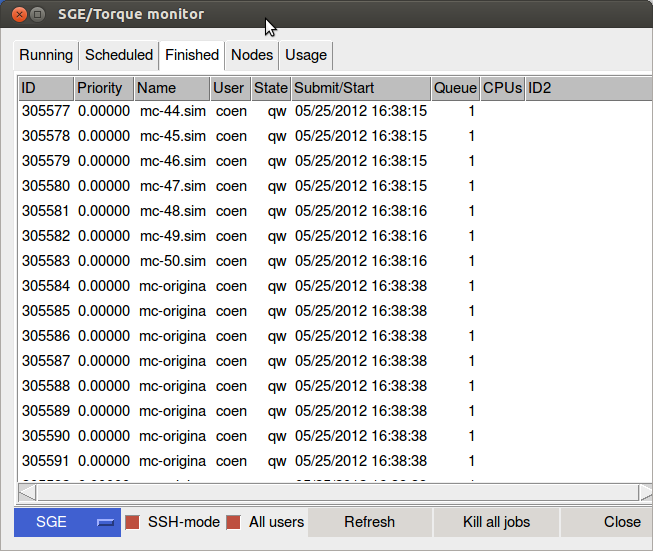
\includegraphics[scale=0.3]{images/Figure3_1_SGEmonitor.png}
    \caption{Job monitor}
\end{figure}

\section{Working with PCluster}
Additionally, Pirana supports the construction of a simple
Windows-based clustering system (PCluster). PCluster allows set up of a cluster using
e.g. PCs of colleagues, and is easy to install on Windows systems.
Please note that this kind of setup is inferior to the clusters
mentioned above in terms of stability and performance. The development of PCluster has now been
discontinued, and no active support will be provided for this
feature. If you still want to try the PCluster, there is a short
manual available upon request.

%%%%%%%%%%%%%%%%%%%%%%%%%%%%%%%%%%%%%%%%%%%%%%%%%%%%%%%%%%%%%%%%%%%%%%%%%%
\chapter{Automated modeling workflow in
Pirana}

\section{Background}\label{background}

An automated workflow alleviates the burden on modeling scientist by
removing the repetitive task of running and evaluating many candidate
models, standardizes the model development between modelers, and
standardize the results reported from such an analysis ultimately
leading to higher quality of PopPK analyses (\emph{Schmidt et al. JPKPD
2014 Aug}). In Pirana (version \textgreater{}= 2.10), such a workflow is
made available, and in this chapter we will walk through an example of
an automated population PK analysis.

\section{Tutorial}

For this chapter, we will use the template model library that is
provided with Pirana, and a (simulated) dataset of an iv-administered
drug also provided with Pirana (\texttt{demo.csv}).

\subsubsection*{Start}

Start Pirana Create a new project folder somewhere on your hard-drive
(or cluster). Browse into this folder (with Pirana). In this folder,
copy the file \texttt{demo.csv} that is included in the Pirana
installation folder (\texttt{Pirana/automod\_library/demo/demo.csv}). In
Pirana, go to \textbf{Tools} --\textgreater{} \textbf{Automated modeling
workflow}.


\subsubsection*{Screen 1: Models and
dataset}

\begin{figure}[htbp]
\centering
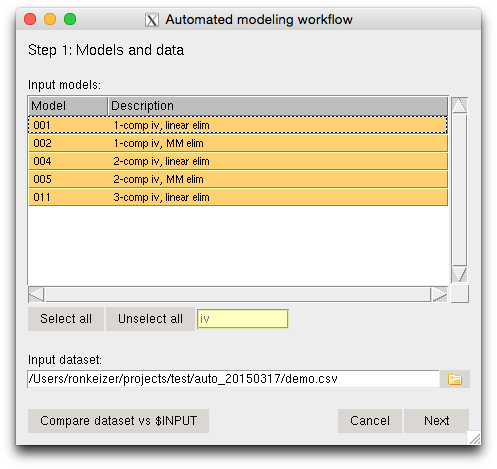
\includegraphics[scale=0.5]{images/screen1.png}
\caption{Screen 1: Models and dataset}
\end{figure}

This screen shows all models available in the library and which can be
selected to be included in the analysis. Use the filter for conveniently
selecting e.g.~only \emph{iv} or only \emph{oral} models. The dataset
should of course be specified as well before you can advance to the next
step. By default, it will use the first \texttt{.csv} file in this
folder (in alphabetic order).

When models and dataset have been selected, you should check whether the
\texttt{\$INPUT} record in the models matches with the headers in the
dataset. For this, click the button \texttt{Compare dataset vs}\$INPUT`.
This will bring up screen shown in figure 2:

\begin{figure}[htbp]
\centering
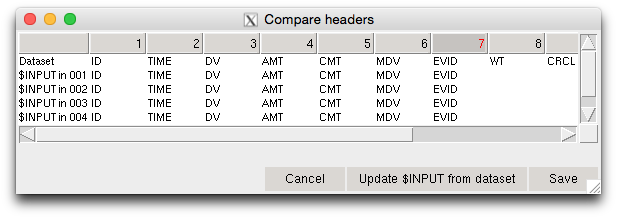
\includegraphics[scale=0.5]{images/compare.png}
\caption{Compare/set input headers}
\end{figure}

If the \texttt{\$INPUT} in the models (shown in rows 2-\ldots{}) does
not match up with the dataset (shown in row 1), you can click the button
\texttt{Update \$INPUT from dataset}. This will create a new \$INPUT
record for all models. After clicking \textbf{Save}, when the models
will be written (in step 3 of the automated analysis), the \$INPUT
records in all models will be changed to the new one. It is left to the
user to make sure that the variables used in the model are still
included in \$INPUT, as there is no extra check in place for that.

For our current analysis, we will select all \emph{iv} models, so filter
on \emph{iv}, and select the remaining models. Update the
\texttt{\$INPUT} records, click \emph{Save} and then \emph{Next} to
advance to the next step.


\subsubsection*{Screen 2: Setting initial parameter
estimates}\label{screen-2-setting-initial-parameter-estimates}

In the second screen, we can set initial parameter estimates, as well as
lower and upper bounds. All parameters are read from the models that
were selected in step 1. The parameter descriptions are defined in the
models as comments to \texttt{\$THETA}, \texttt{\$OMEGA}, and
\texttt{\$SIGMA} blocks, like e.g.

\begin{figure}[htbp]
\centering
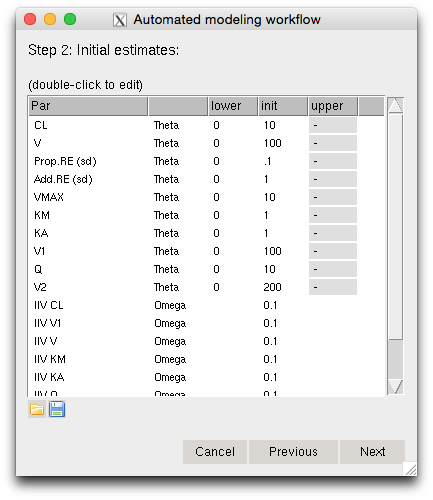
\includegraphics[scale=0.5]{images/screen2.png}
\caption{Screen 2: Initial parameter estimates}
\end{figure}

\begin{verbatim}
$THETA
(0, 5, 100); CL
(0, 5, 100); V

$OMEGA
(0.1); CL
(0.1); V

$SIGMA
0.05 ; proportional error
\end{verbatim}

\emph{Note:} At current, correlations in \$OMEGA and \$SIGMA cannot be
specified for an automated analysis. I.e. only the diagonal elements of
\$OMEGA and \$SIGMA can be specified in the template models if you want
to update them in this step. You can still include models that have full
\$OMEGA or \$SIGMA blocks as template model, however you cannot provide
descriptions (as comments) to the parameters in the block, and you
cannot update them in this step of the analysis.

The two buttons below the parameter grid can be used to save and
(re-)load parameter definitions to file.

For our analysis, let's leave the parameters as they are. Click
\textbf{Next} to advance to the next step.


\subsubsection*{Screen 3: Folders}\label{screen-3-folders}

\begin{figure}[htbp]
\centering
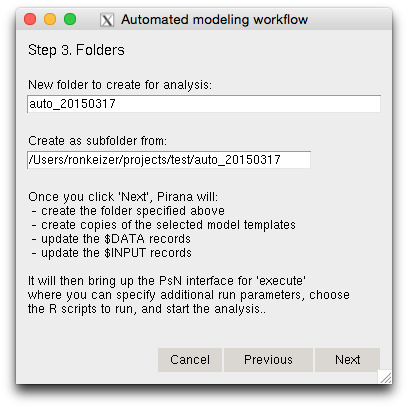
\includegraphics[scale=0.5]{images/screen3.png}
\caption{Screen 3: Folders}
\end{figure}

In this screen we can specify where to create the new models and run the
analysis. By default it will generate a new folder name based on the
current date, and as a subfolder from the current folder in Pirana. This
screen also lists the actions that Pirana will perform once you click
\emph{Next}.

Let's use the defaults and click \emph{Next}.


\subsubsection*{Screen 4: PsN dialog}\label{screen-4-psn-dialog}

\begin{figure}[htbp]
\centering
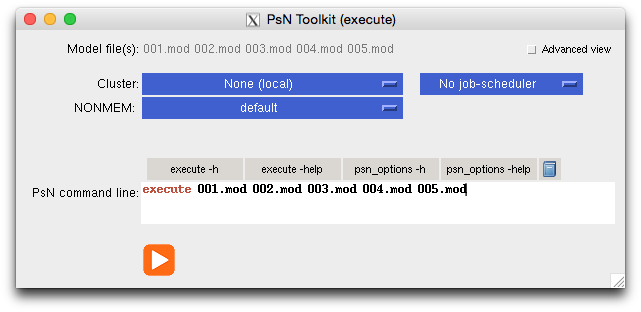
\includegraphics[scale=0.5]{images/psn_simple.png}
\caption{Screen 4: PsN}
\end{figure}

Pirana should now have switched automatically to the new folder where
you will see the newly generated models. Pirana will also automatically
bring up the PsN \texttt{execute} dialog. In this dialog, if you switch
to \textbf{Advanced view}, you can select which R script(s) to run after
all runs have been completed to generate goodness-of-fit plots. Click
the \emph{folder} icons next to the R scripts textboxes to select R
scripts (or batch files) to run after (or before) the analysis (figure
6).

\begin{figure}[htbp]
\centering
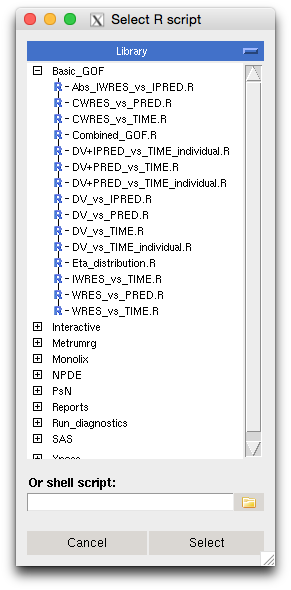
\includegraphics[scale=0.5]{images/run_r.png}
\caption{Select R script}
\end{figure}

For our analysis, we will select the \textbf{Basic GOF plots as single
doc} from the \texttt{Reports} folder to create GOF plots for all
models. The graphical report will automatically be opened, but is also
available from the \emph{Reports} tab on the right.

If you have not selected R scripts to be executed automatically after
the analysis has completed, you can still create them afterwards by
selecting the runs and running any R script from the \textbf{R} tab on
the right side of the Pirana window.

Besides the graphical report, Pirana can generate a \emph{numeric}
report for the analysis, including e.g.~OFVs, basic run information and
parameter estimates. This document is not generated automatically but
has to be requested manually after the analysis is complete: Make sure
Pirana is still in the folder where the analysis was run, and then go to
\textbf{Tools} --\textgreater{} \textbf{Automated modeling workflow}
--\textgreater{} \textbf{Report}. On the first page you will see an
overview of all models included in the analysis and their respective
OFV, AIC and BIC (figure 7). The subsequent pages includes information
on each individual run in the analysis.

\begin{figure}[htbp]
\centering
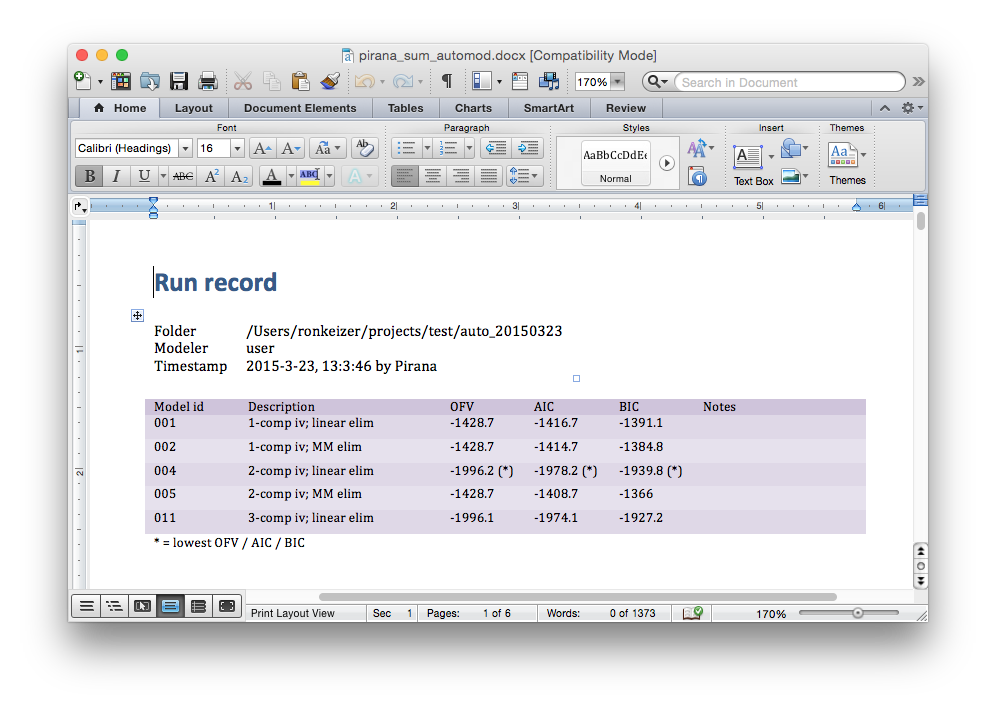
\includegraphics[scale=0.5]{images/report.png}
\caption{Report in Word}
\end{figure}



%%%%%%%%%%%%%%%%%%%%%%%%%%%%%%%%%%%%%%%%%%%%%%%%%%%%%%%%%%%%%%%%%%%%%%%%%%
\chapter{cPirana}
cPirana is a simple, `lite' version of Pirana that runs on the Unix command line.
There are several reasons that we think cPirana is a useful addition to our primary software product.
Over the years we have encountered many --usually more experienced--
modelers that prefer to work from the command line. We still think a user interface (be it graphical or
console-based) can greatly increase productivity and make the modeling process
easier in general. For those modelers, we hope cPirana is a welcome addition to their workflow.

\vspace{10pt}

\noindent Secondly, while working on cluster through a slow internet connection, the interface may become slow.
Version 2.7.0 included already many speed improvements that improves working on slow connections. However,
e.g. when traveling, one might be only interested in making a few small code changes and restart a model.
If a computer with Pirana is not available, or if the internet connection is very slow, you probably will still
be able to login to your cluster over ssh. If cPirana is installed on this cluster, you will have the ability to
use most Pirana functions directly from the command line interface.

\vspace{10pt}

\noindent Finally, already from our earliest versions of Pirana, we intended to extend the implementation
of Pirana to smartphone or tablets, allowing for increased mobility
and connectivity. While the implementation of a true dedicated Pirana
app is currently beyond the capacity of our small development team, cPirana
actually offers this possibility: if cPirana is installed on the Linux
cluster that runs NONMEM and PsN, the user can connect from a tablet
or smartphone using specialized ssh-apps (such as `Prompt' on the
iPad), to connect.

\vspace{10pt}

\begin{figure}[hbt] \centering
    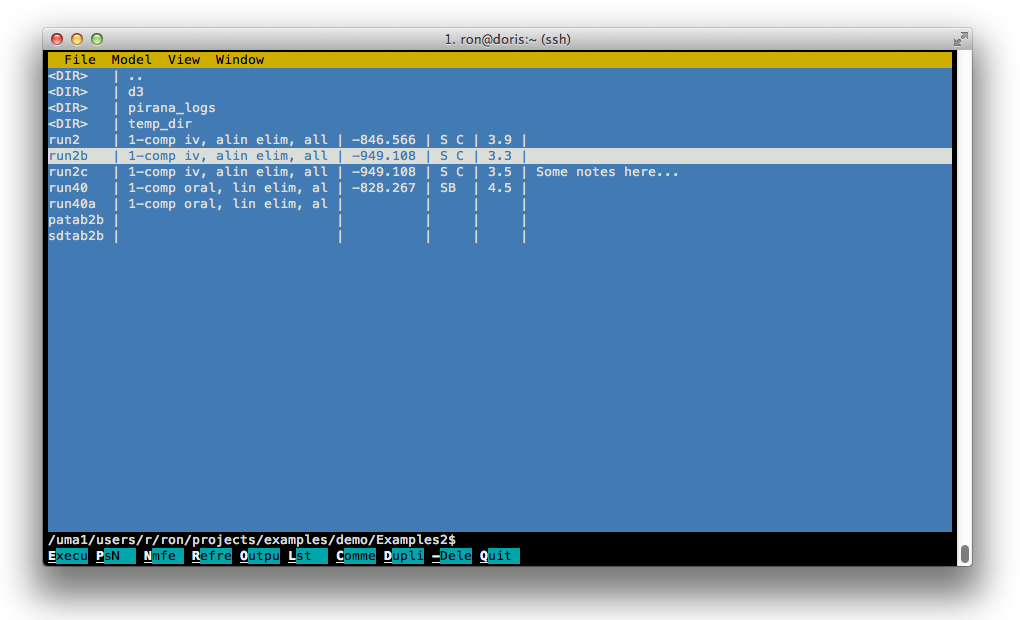
\includegraphics[scale=0.3]{images/cpirana_main.png}
    \caption{cPirana interface example}
\end{figure}


\section{Installing cPirana}

\subsection{Starting cPirana}
Copy the contents of the linux installation zip-file file to a location on your system. Pirana is started using the command (assuming you installed it in the folder /pirana inside your home folder):

\begin{lstlisting}
perl ~/pirana/cpirana.pl
\end{lstlisting}

cPirana will use the current folder as it's working folder. To make cPirana more easily accessible, add it as an alias to your .bashrc file, i.e.

\begin{lstlisting}
alias cpirana="perl ~/pirana/cpirana.pl"
\end{lstlisting}

Now you can browse to any folder, and start the program from there
using the {\ttfamily cpirana} command.

\vspace{10pt}
\noindent \scriptsize \textcolor{Blue}{Tip:} \textcolor{Grey} The manual section for cPirana is currently in development. Please check back regularly.
\normalsize


%%%%%%%%%%%%%%%%%%%%%%%%%%%%%%%%%%%%%%%%%%%%%%%%%%%%%%%%%%%%%%%%%%%%%%%%%%
\newpage  % one page left blank intentially
\thispagestyle{empty}
\mbox{}

\chapter{Validation}
Of course, the information gained from NONMEM or auxiliary tools must be
reliable and accurate. Validation of these tools is therefore an important consideration.
The main aim of Pirana is to provide overviews of modeling results and
providing interfaces to other software (NONMEM, PsN, R, Xpose). As such, Pirana does not perform many calculations of its own. However,
Pirana does performs data parsing, formatting and reporting, i.e. in the creation of run reports.

\noindent The Pirana development team has developed tools that perform a validation of parts of this
ecosystem. At current, we have two tools available:

\begin{description}
\item[valpsn] is a command-line tool that performs a
  series of pre-specified numerical tests, based on output from PsN
  tools. In the comparisons, the output from the specific PsN version
  that is to be validated (`test'-output) is compared to previously
  obtained output from a PsN version that is trusted, or has been
  validated in other ways (`reference'-output). The tools is
  scriptable, and includes R-scripts to perform the numerical
  comparison. It is however completely flexible, i.e. it allows custom
  R-scripts to be provided to perform the tests. The tool is currently
  not yet available from the Pirana website but can be supplied upon request.
\item[valpirana] is a command-line tool that perform a
  series of numerical test on the parameter estimates outputted by
  Pirana. The parameters ('test') are compared to those extracted by
  PsN's sumo tool (`reference'), for a user-specified library of
  models and modeling result files. This tool therefore solely focuses
  on Pirana and PsN's algorithms extraction of parameter estimates
  from NONMEM output files. Ultimately, this is Pirana's key feature,
  since Pirana does not perform many calculations, but is primarily a
  tool to generate overviews of results and allow the modeler to
  interpret results easier. The tool is currently
  not yet available from the Pirana website but can be supplied upon request.
\end{description}

\noindent Note that both validation tools can be used to validate NONMEM as
well, e.g. if the reference output is obtained from a new, to be
validated, NONMEM version and compared to previously execute NONMEM
runs with a reference NONMEM version.

\vspace{20pt}
\noindent \textbf{IMPORTANT}: We do not claim any responsibility for the outcome
or validity of the validation analyeses obtained using these
tools. For example, we cannot guarantee that regulatory autharities accept
particular validations performed with these tools, nor do we claim the correctness of the validation results.
Please align intended validation procedure with the relevant authorities beforehand.

\section{Pirana validation tool}
While a few models and model outputs are supplied with the Pirana
validation tool, it is expected that the user provides a library of
models and NONMEM output files (usually .lst or .res files). The
Pirana validation tool expects a specific directory structure:

\begin{lstlisting}
\val_library
   - \res1
        - \model
   - \res2
   - \res3
\end{lstlisting}

\noindent The valpirana Perl script is invoked from the command line, using
e.g.:

\begin{lstlisting}
perl valpirana.pl -ini=val_pirana20130224.ini
\end{lstlisting}

ValPirana will then read the ini-file, and loop (alphabetically)
through all folders in the folder specified in the ini-file. In each
folder, it will extract all parameter estimates and standard error
estimates (if available) using Pirana's internal NONMEM output parsing
routines. It will then run PsN's 'sumo' command, and store the
parameters outputted by PsN to memory as well. These will then be
compared, allowing for a pre-specified tolerance due to rounding.
The ini-file should be specified similar to:

\begin{lstlisting}
[general]
mod=mod
lst=lst
psn_dir=/usr/bin/
pirana_modules=/shared/val/pirana_modules_270
tol=

[lib1]
folder=/shared/val/valpirana_

[lib2]  # Optionally, specify multiple libraries
folder=
\end{lstlisting}

\subsubsection*{Pirana pre-release validation}
Before every Pirana release from version 2.4.0 upwards we used
(predecessors of) the valpirana tool to check that the parameter
estimates that Pirana extracts from NONMEM output files are exactly
the same as the ones reported by PsN's sumo command. For this
validation procedure we gathered more than 50 model and results files
from multiple modeling groups and many different modelers. While we cannot share the
model and output in the validation library, if you
would like a report of the validation procedure, please contact us.

\section{PsN validation tool}
The PsN validation tool compares output from a `test'-installation of
PsN, with output from a trusted (previous) PsN installation. Tests can
be implemented for any of the tools in PsN (e.g. execute, bootstrap,
vpc, etc), and multiple tests can be performed for each tool
(recommended). The tests to be performed are specified in a setup file. Customizable
R scripts are used to perform the actual validation step for the tool. Every validation run is started by invoking the valpsn command:

\begin{lstlisting}
./valpsn ex1\_20130201.ini
\end{lstlisting}

\noindent This bash script invokes the main perl script that acutally performs the
validation. The script will read in the configuration file, and will
perform all the specified validation elements in the sequence
specified in the configuration file. The specific tests in the
validation run are all implemented in R scripts, and should output
SUCCESS or FAILURE. For every PsN tool a test script is provided with
the tool, but the user is encouraged to write custom scripts.
More info is available in the specific manual for this tool (available upon request).

%%%%%%%%%%%%%%%%%%%%%%%%%%%%%%%%%%%%%%%%%%%%%%%%%%%%%%%%%%%%%%%%%%%%%%%%%%
\chapter{Endnotes}
\section{Acknowledgements} Many Pirana users are recognized for their
valuable suggestions and bug-reports, especially those in the Uppsala
and Amsterdam pharmacometrics groups.

\section{Bug reporting / suggestions}
If you find any bugs, please report them at the support section of our
website (http://www.pirana-software.com). A ticket will be created,
and we will get back to you as soon as possible. Please be as specific
as you can about the issue and report version number, system
characteristics, and if relevant provide screenshots and model/results
files. Requests of tips for further improvement of Pirana are very
welcome as well and can also be reported at the support section.

\section{Disclaimer} This software is provided under both an academic
and a commercial license. It is distributed on an `as is' basis,
without warranty of any kind. Your use of the software is at your sole
risk, and the authors cannot be held liable for any harm, inflicted
upon your system by this program. Any decision made on the basis of
output produced by Pirana is entirely your own responsibility. The
user is referred to the license for more information

\normalsize
